%% LyX 2.3.3 created this file.  For more info, see http://www.lyx.org/.
%% Do not edit unless you really know what you are doing.
\documentclass[11pt,a4paper,english]{desearticle_1col}
%\documentclass[11pt,a4paper,english]{desearticle}
\usepackage{mathptmx}
\usepackage{helvet}
\usepackage{courier}
\renewcommand{\familydefault}{\rmdefault}
\usepackage[latin9]{inputenc}
\usepackage{fancyhdr}
\pagestyle{fancy}
\usepackage{float}
\usepackage{booktabs}
\usepackage{graphicx}
\usepackage{algorithm}
\usepackage{algorithmic}
\usepackage{listings}
\usepackage{xcolor}
\usepackage{listings}
\usepackage{xcolor}
\usepackage{lipsum} % For sample text
\usepackage{amsmath}
\usepackage{array}
\usepackage{geometry}
\usepackage{booktabs}
\usepackage{geometry}
\usepackage{adjustbox}
\usepackage{tikz}
\usepackage{float}
\usetikzlibrary{shapes.geometric, arrows}
\usepackage{svg}

\tikzstyle{startstop} = [rectangle, rounded corners, minimum width=3cm, minimum height=1cm,text centered, draw=black, fill=red!30]
\tikzstyle{process} = [rectangle, minimum width=3cm, minimum height=1cm, text centered, draw=black, fill=orange!30]
\tikzstyle{decision} = [diamond, minimum width=3cm, minimum height=1cm, text centered, draw=black, fill=green!30]
\tikzstyle{arrow} = [thick,->,>=stealth]

\usepackage{longtable}
\usetikzlibrary{shapes.geometric, arrows}
\geometry{left=1in, right=1in, top=1in, bottom=1in}
\definecolor{codebackground}{rgb}{0.95,0.95,0.95}
\definecolor{codegreen}{rgb}{0,0.6,0}
\definecolor{codeblue}{rgb}{0,0,0.8}
\definecolor{codegray}{rgb}{0.5,0.5,0.5}
\definecolor{codepurple}{rgb}{0.6,0,0.8}

\lstdefinestyle{mystyle}{
	backgroundcolor=\color{codebackground},   
	commentstyle=\color{codegreen},
	keywordstyle=\color{codeblue},
	numberstyle=\tiny\color{codegray},
	stringstyle=\color{codepurple},
	basicstyle=\ttfamily\footnotesize,
	breakatwhitespace=false,         
	breaklines=true,                 
	captionpos=b,                    
	keepspaces=true,                 
	numbers=left,                    
	numbersep=5pt,                  
	showspaces=false,                
	showstringspaces=false,
	showtabs=false,                  
	tabsize=2
}

\lstset{style=mystyle}
\makeatletter

%%%%%%%%%%%%%%%%%%%%%%%%%%%%%% LyX specific LaTeX commands.
\pdfpageheight\paperheight
\pdfpagewidth\paperwidth

%% Because html converters don't know tabularnewline
\providecommand{\tabularnewline}{\\}

%%%%%%%%%%%%%%%%%%%%%%%%%%%%%% User specified LaTeX commands.
\Author{Vaibhav Shatalwar}
\Afil{DESE, IISc}
\Journal{Processor Systems Design}
\Month{Aug-Dec}
\Year{2024}

\makeatother

\usepackage{babel}
\begin{document}
\title{{\huge{}Lab Exercise-3}}
\maketitle
\begin{abstract}
The objective of this Lab exercise is to implement a Pipelined RISC-V Processor with 
Instruction Cache.
\end{abstract}

%\section{Introduction}
%In this experiment, we are using L298 motor driver to drive
%inductive loads such as relays, solenoids, DC and
%stepping motors. The L298 is an integrated monolithic circuit in a 15-
%lead Multiwatt and PowerSO20 packages.Two enable inputs are provided to
%enable or disable the device independently of the input signals. The emitters of the lower transistors of
%each bridge are connected together and the corresponding external terminal can be used for the connection of an external sensing resistor.
%
%
%This section provides an introduction to the experiment. Discuss the
%need for the experiment and how it will be executed? What will be 
%learned from this experiment? What are the necessary background literature
%that you have referred? In this section you will include citation
%to the references like datasheets, papers, articles, notes etc. Build
%up you list of references in a .bib file in bibtex format. Load the
%bibtex into the ``Bibtex generated bibliography'' template at the
%end of this article. The references can then be cited in the text
%of the article. I will cite two references here that will automatically
%get sorted and listed at the end in the references section. \cite{lp3w}
%is an arbitrary book reference and \cite{LM741} is a reference to
%the data sheet of LM 741 op-amp.

\section{Processor Design}

Design and Implement a 5-stage Pipelined RISC-V processor on Digilent BASYS3 
FPGA Board. Target Device is Xilinx Artix-7 XC7A35T- ICPG236C (Family Artix-7, Part 
XC7A35T, Package CPG236, Speed Grade -1).

The Processor is a 32-bit RISC-V Processor. The processor should support basic arithmetic-logic instructions, branch instructions, \texttt{lui}, load-store instructions, and jump instructions. Atomic instructions, \texttt{auipc} and CSR instructions need not be supported. Implement hazard detection and forwarding (from EX, MEM, and WB stage outputs). Implement the Stall unit for load, and branch instructions.

\subsection{Design Requirements}

\begin{itemize}
	\item 5-stage pipeline: Fetch, Decode, Execute, Memory, and Write-back
	\item Support for basic arithmetic-logic instructions, branch, \texttt{lui}, and load-store instructions
	\item Hazard detection and forwarding logic
	\item Stall unit for load and branch instructions
	\item Instruction cache implementation (direct-mapped with a block size of four words)
	\item Block RAM for main instruction memory
	\item No burst transfer for cache filling
	\item No support for \texttt{atomic}, \texttt{auipc}, and \texttt{CSR} instructions
	\item Aligned transfer for word, half-word, and byte data
	\item No data cache, data access via data memory
\end{itemize}

\subsection{Processor Testing}

Test the processor with a suitable algorithm, using a procedure call. The program can be written in C, and the corresponding assembly or binary code should be used for testing.

\subsection{Design Flow}

\begin{enumerate}
	\item Design the Datapath block schematic.
	\item HDL coding for the RISC-V processor.
	\item Implement hazard detection and forwarding units.
	\item Implement stall logic for load and branch instructions.
	\item Create the instruction cache using block RAM on the FPGA.
	\item Use IO Constraints and Timing Constraints to optimize performance.
	\item Perform Timing Analysis and Timing simulation with a proper testbench.
	\item Generate binary code from C program and load it into memory.
	\item Implement the design on BASYS3 FPGA Board.
\end{enumerate}

\subsection{Submission Requirements}

Submit the following:
\begin{itemize}
	\item Block schematic of the Datapath design.
	\item State diagram of the controller (if any).
	\item Source Verilog codes.
	\item IO and Timing Constraint files.
	\item Timing Report.
	\item Resource utilization.
	\item Software code for testing.
\end{itemize}


%\section{Introduction}
%The processor has basic five stages for computation includes fetch,decode,execution,memory and write back.
%Additionally it has prefetch stage added to increase the speed. It supports minimal operations like arithmetic,logical and branch.
%\subsection{Instruction memory:}
%\begin{align*}
%	\text{Program Counter (PC) width} &= 16 \text{ bits}\\
%	\Rightarrow\qquad \text{Address width} &= 16 \text{ bits}
%\end{align*}
%\subsection{Data Memory:}
%The Data Address width is 16 bits.
%
%\begin{align*}
%	\text{Data Address width} &= 16 \text{ bits}
%\end{align*}
%
%\subsection{Register File:}
%The register file consists of 8 registers, labeled R0-R7, each with a width of 16 bits. The register file has:
%
%\begin{itemize}
%	\item 2 asynchronous read ports
%	\item 1 synchronous write port
%\end{itemize}
%
%Additionally, register R0 is hardwired to always contain the value 0.
%
%\begin{align*}
%	R0 &= 0
%\end{align*}
%\subsection{Arithmetic Logic Unit (ALU) Specifications}
%
%The ALU is a 16-bit unit that supports the following instructions:
%
%\begin{itemize}
%	\item Arithmetic:
%	+ ADD
%	+ SUB
%	\item Logical:
%	+ AND
%	+ OR
%	+ XOR
%	+ NOT
%	\item Shift:
%	+ LSL (Logical Shift Left)
%	+ LSR (Logical Shift Right)
%	+ ASR (Arithmetic Shift Right)
%\end{itemize}
%
%In addition to the result, the ALU generates the following flags for branch type instructions:
%
%\begin{itemize}
%	\item Greater than (gt)
%	\item Less than (lt)
%	\item Zero (z)
%\end{itemize}
%
%%\subsection{Arithmetic Logic Unit (ALU) Specifications}
%%
%%\begin{table}[h]
%%	\centering
%%	\begin{tabular}{|l|c|}
%%		\hline
%%		\textbf{Instruction Type} & \textbf{Instructions} \\
%%		\hline
%%		Arithmetic & ADD, SUB \\
%%		\hline
%%		Logical & AND, OR, XOR, NOT \\
%%		\hline
%%		Shift & LSL, LSR, ASR \\
%%		\hline
%%	\end{tabular}
%%	\caption{ALU Instructions}
%%\end{table}
%%
%%\begin{table}[h]
%%	\centering
%%	\begin{tabular}{|l|c|}
%%		\hline
%%		\textbf{Flag} & \textbf{Description} \\
%%		\hline
%%		gt & Greater than \\
%%		\hline
%%		lt & Less than \\
%%		\hline
%%		z & Zero \\
%%		\hline
%%	\end{tabular}
%%	\caption{ALU Flags}
%%\end{table}
%
%\subsection{Instruction Register (IR) and Instruction Pre-fetch Register (IPR)}
%
%The Instruction Register (IR) and Instruction Pre-fetch Register (IPR) are 16 bits wide registers that are written to upon receiving enable signals.
%
%\subsubsection{Instruction Register (IR)}
%
%The Instruction Register (IR) holds the instruction that is currently being executed.
%
%\subsubsection{Instruction Pre-fetch Register (IPR)}
%
%The Instruction Pre-fetch Register (IPR) holds the next instruction to be executed.
%
%
%\subsection{Sign Extension Module}
%
%The Sign Extension Module is a digital circuit that performs the following operation:
%
%\begin{itemize}
%	\item Accepts a 7-bit immediate/offset field as input
%	\item Generates a 16-bit output by sign-extending the most significant bit (MSB) to all upper positions
%\end{itemize}


\section{Instruction Set Architecture and Instruction Format}

%\begin{table}[h!]
%	\centering
%	\begin{tabular}{|>{\centering\arraybackslash}m{2.5cm}|>{\centering\arraybackslash}m{2.5cm}|m{7cm}|}
%		\hline
%		\textbf{Instruction} & \textbf{Assembly Operation} & \textbf{Description} \\
%		\hline
%		LD & LD R1 \#imm(R0) & R1 $\leftarrow$ [R0+imm] \\
%		\hline
%		ST & ST R2 \#imm(R0) & [R0+imm] $\leftarrow$ R2 \\
%		\hline
%		ADDI & ADDI R1 \#imm(R0) & R1 = R0 + imm \\
%		\hline
%		ADD & ADD R1, R2, R3 & R1 = R2 + R3 \\
%		\hline
%		SUB & SUB R1, R2, R3 & R1 = R2 - R3 \\
%		\hline
%		AND & AND R1, R2, R3 & R1 = R2 \& R3 \\
%		\hline
%		OR & OR R1, R2, R3 & R1 = R2 $|$ R3 \\
%		\hline
%		NOT & NOT R1, R2 & R1 = $\sim$R2 \\
%		\hline
%		XOR & XOR R1, R2, R3 & R1 = R2 $\oplus$ R3 \\
%		\hline
%		LSL & LSL R1, R2, R3 & R1 = R2 $\ll$ R3 \\
%		\hline
%		LSR & LSR R1, R2, R3 & R1 = R2 $\gg$ R3 \\
%		\hline
%		ASR & ASR R1, R2, R3 & R1 = R2 $\ggg$ R3 \\
%		\hline
%		BGT & BGT R1, R2, \#Offset & Branch to PC+1+Offset if R1 $>$ R2 \\
%		\hline
%		BLT & BLT R1, R2, \#Offset & Branch to PC+1+Offset if R1 $<$ R2 \\
%		\hline
%		BNZ & BNZ R1, \#Offset & Branch to PC+1+Offset  if R1 $\neq$ 0 \\
%		\hline
%		HALT & HALT & Halts execution \\
%		\hline
%	\end{tabular}
%	\caption{Instruction Set Assembly Operations}
%\end{table}


\subsection{R-Type Instructions (Arithmetic and Logic)}

\noindent\textbf{Operation}: Rd = Rs1 op Rs2 \\
\textbf{Assembly}: \textit{Instr Rd Rs1 Rs2} \\
\textbf{Format}: \\

\begin{tabular}{|c|c|c|c|c|c|}
	\hline
	\textbf{Funct7} & \textbf{Rs2} & \textbf{Rs1} & \textbf{Funct3} & \textbf{Rd} & \textbf{Opcode} \\
	\hline
	\multicolumn{1}{|p{2cm}|}{\centering \textbf{31-25}} & 
	\multicolumn{1}{|p{2cm}|}{\centering \textbf{24-20}} & 
	\multicolumn{1}{|p{2cm}|}{\centering \textbf{19-15}} & 
	\multicolumn{1}{|p{2cm}|}{\centering \textbf{14-12}} & 
	\multicolumn{1}{|p{2cm}|}{\centering \textbf{11-7}} & 
	\multicolumn{1}{|p{2cm}|}{\centering \textbf{6-0}} \\
	\hline
\end{tabular}

\vspace{0.5cm}

For all R-type instructions, Opcode = 0110011 \\

\vspace{0.5cm}

\noindent\begin{longtable}{|c|c|c|c|}
	\hline
	\textbf{Instruction} & \textbf{Operation} & \textbf{Funct3} & \textbf{Funct7} \\
	\hline
	ADD & $Rd = Rs1 + Rs2$ & 000 & 0000000 \\
	\hline
	SUB & $Rd = Rs1 - Rs2$ & 000 & 0100000 \\
	\hline
	AND & $Rd = Rs1 \,\&\, Rs2$ & 111 & 0000000 \\
	\hline
	OR  & $Rd = Rs1 \,|\, Rs2$  & 110 & 0000000 \\
	\hline
	XOR & $Rd = Rs1 \oplus Rs2$ & 100 & 0000000 \\
	\hline
	SLL & $Rd = Rs1 \ll Rs2$ & 001 & 0000000 \\
	\hline
	SRL & $Rd = Rs1 \gg Rs2$ & 101 & 0000000 \\
	\hline
	SRA & $Rd = Rs1 \ggg Rs2$ & 101 & 0100000 \\
	\hline
\end{longtable}



\subsection{Load}
\noindent\textbf{Operation}: Rd = mem[Rs1 + Imm] \\
\textbf{Assembly}: \textit{Instr Rd Rs1 Imm} \\
\textbf{Format}: \\

\begin{tabular}{|c|c|c|c|c|}
	\hline
	\textbf{Immediate} & \textbf{Rs1} & \textbf{Funct3} & \textbf{Rd} & \textbf{Opcode} \\
	\hline
	\multicolumn{1}{|p{3cm}|}{\centering \textbf{31-20}} & 
	\multicolumn{1}{|p{2cm}|}{\centering \textbf{19-15}} & 
	\multicolumn{1}{|p{1.5cm}|}{\centering \textbf{14-12}} & 
	\multicolumn{1}{|p{2cm}|}{\centering \textbf{11-7}} & 
	\multicolumn{1}{|p{1.5cm}|}{\centering \textbf{6-0}} \\
	\hline
\end{tabular}

\vspace{0.5cm}

For all load instructions, Opcode = 0000011 \\

\vspace{0.5cm}

\noindent\begin{longtable}{|c|c|c|}
	\hline
	\textbf{Instruction} & \textbf{Operation} & \textbf{Funct3} \\ 
	\hline
	LW  & Loads word                           & 010 \\ 
	\hline
	LH  & Loads half word (sign extended)       & 001 \\ 
	\hline
	LHU & Loads half word (zero extended)       & 101 \\ 
	\hline
	LB  & Loads byte (sign extended)            & 000 \\ 
	\hline
	LBU & Loads byte (zero extended)            & 100 \\ 
	\hline
\end{longtable}

\subsection{Store}
\noindent\textbf{Operation}: mem[Rs1 + Imm] = Rs2 \\
\textbf{Assembly}: \textit{Instr Rs2 Rs1 Imm} \\
\textbf{Format}: \\

\begin{tabular}{|c|c|c|c|c|c|}
	\hline
	\textbf{Imm[12:6]} & \textbf{Rs2} & \textbf{Rs1} & \textbf{Funct3} & \textbf{Imm[5:1]} & \textbf{Opcode} \\
	\hline
	\multicolumn{1}{|p{2cm}|}{\centering \textbf{31-25}} & 
	\multicolumn{1}{|p{2cm}|}{\centering \textbf{24-20}} & 
	\multicolumn{1}{|p{2cm}|}{\centering \textbf{19-15}} & 
	\multicolumn{1}{|p{2cm}|}{\centering \textbf{14-12}} & 
	\multicolumn{1}{|p{2cm}|}{\centering \textbf{11-7}} & 
	\multicolumn{1}{|p{2cm}|}{\centering \textbf{6-0}} \\
	\hline
\end{tabular}

\vspace{0.5cm}

For all store instructions, Opcode = 0100011 \\

\vspace{0.5cm}

\noindent\begin{longtable}{|c|c|c|}
	\hline
	\textbf{Instruction} & \textbf{Operation} & \textbf{Funct3} \\
	\hline
	SW  & Stores word          & 000 \\
	\hline
	SH  & Stores half word     & 001 \\
	\hline
	SB  & Stores byte          & 010 \\
	\hline
\end{longtable}
\subsection{ADDI}
\noindent\textbf{Operation}: Rd = Rs1 + Imm \\
\textbf{Assembly}: \textit{ADDI Rd Rs1 Imm} \\
\textbf{Format}: \\

\begin{tabular}{|c|c|c|c|c|c|c|}
	\hline
	\textbf{Immediate} & \textbf{Rs1} & \textbf{Funct3} & \textbf{Rd} & \textbf{Opcode} \\ 
	\hline
	\multicolumn{1}{|p{2cm}|}{\centering \textbf{31-20}} & 
	\multicolumn{1}{|p{2cm}|}{\centering \textbf{19-15}} & 
	\multicolumn{1}{|p{2cm}|}{\centering \textbf{14-12}} & 
	\multicolumn{1}{|p{2cm}|}{\centering \textbf{11-7}} & 
	\multicolumn{1}{|p{2cm}|}{\centering \textbf{6-0}} \\ 
	\hline
\end{tabular}

\vspace{0.5cm}

For all immediate instructions, Opcode = 0010011 \\

\vspace{0.5cm}

\noindent\begin{longtable}{|c|c|c|}
	\hline
	\textbf{Instruction} & \textbf{Operation} & \textbf{Funct3} \\ 
	\hline
	ADDI & Adds immediate to register & 000 \\ 
	\hline
\end{longtable}


\subsection{Branch Type Instructions}

\noindent\textbf{Operation}: Goes to instruction at PC + Imm\textsubscript{shifted} if branching condition is satisfied. \\
\textbf{Assembly}: \textit{Instr Rs1 Rs2 Imm} \\
\textbf{Format}: \\

\begin{table}[h!]
	\centering
	\adjustbox{max width=\textwidth}{
		\begin{tabular}{|c|c|c|c|c|c|c|c|}
			\hline
			\textbf{Imm[12]} & \textbf{Imm[10:5]} & \textbf{Rs2} & \textbf{Rs1} & \textbf{Funct3} & \textbf{Imm[4:1]} & \textbf{Imm[11]} & \textbf{Opcode} \\
			\hline
			\multicolumn{1}{|p{2cm}|}{\centering \textbf{31}} & 
			\multicolumn{1}{|p{2cm}|}{\centering \textbf{30-25}} & 
			\multicolumn{1}{|p{2cm}|}{\centering \textbf{24-20}} & 
			\multicolumn{1}{|p{2cm}|}{\centering \textbf{19-15}} & 
			\multicolumn{1}{|p{2cm}|}{\centering \textbf{14-12}} & 
			\multicolumn{1}{|p{2cm}|}{\centering \textbf{11-8}} & 
			\multicolumn{1}{|p{2cm}|}{\centering \textbf{7}} & 
			\multicolumn{1}{|p{2cm}|}{\centering \textbf{6-0}} \\
			\hline
		\end{tabular}
	}
	\caption{Format of Branch Type Instructions}
\end{table}


\vspace{0.5cm}

For all branch instructions, Opcode = 1100011 \\

\vspace{0.5cm}

\noindent\begin{longtable}{|c|c|c|}
	\hline
	\textbf{Instruction} & \textbf{Operation} & \textbf{Funct3} \\
	\hline
	BEQ & Goes to branch target if Rs1 = Rs2  & 000 \\
	\hline
	BNE & Goes to branch target if Rs1 $\neq$ Rs2  & 001 \\
	\hline
	BLT & Goes to branch target if Rs1 $<$ Rs2  & 100 \\
	\hline
	BGE & Goes to branch target if Rs1 $\geq$ Rs2  & 101 \\
	\hline
\end{longtable}

\subsection{LUI}
\noindent\textbf{Operation}: Loads an immediate value into the upper 20 bits of the destination register, setting the lower 12 bits to zero. \\
\textbf{Assembly}: \textit{LUI Rd Imm} \\
\textbf{Format}: \\

\begin{tabular}{|c|c|c|}
	\hline
	\textbf{Imm[31:12]} & \textbf{Rd} & \textbf{Opcode} \\
	\hline
	\multicolumn{1}{|p{4cm}|}{\centering \textbf{31-12}} & 
	\multicolumn{1}{|p{2cm}|}{\centering \textbf{11-7}} & 
	\multicolumn{1}{|p{2cm}|}{\centering \textbf{6-0}} \\
	\hline
\end{tabular}

\vspace{0.5cm}

For all \textbf{LUI} instructions, \textit{Opcode = 0110111}.

\subsection{JAL}
\noindent\textbf{Operation}: Goes to instruction at PC + Imm\textsubscript{shifted} and stores the address of the next instruction (i.e., PC + 4) in the destination register. \\
\textbf{Assembly}: \textit{JAL Rd Imm} \\
\textbf{Format}: \\

\begin{tabular}{|c|c|c|c|c|c|}
	\hline
	\textbf{Imm[20]} & \textbf{Imm[10:1]} & \textbf{Imm[11]} & \textbf{Imm[19:12]} & \textbf{Rd} & \textbf{Opcode} \\
	\hline
	\multicolumn{1}{|p{2cm}|}{\centering \textbf{31}} & 
	\multicolumn{1}{|p{2cm}|}{\centering \textbf{30-21}} & 
	\multicolumn{1}{|p{2cm}|}{\centering \textbf{20}} & 
	\multicolumn{1}{|p{2cm}|}{\centering \textbf{19-12}} & 
	\multicolumn{1}{|p{2cm}|}{\centering \textbf{11-7}} & 
	\multicolumn{1}{|p{2cm}|}{\centering \textbf{6-0}} \\
	\hline
\end{tabular}

\vspace{0.5cm}

For all JAL instructions, Opcode = 1101111 \\

\vspace{0.5cm}
\subsection{JALR}
\noindent\textbf{Operation}: Goes to instruction at Rs1+Imm and stores the address of the next instruction (i.e., PC + 4) in the destination register. \\
\textbf{Assembly}: \textit{JALR Rd Rs1 Imm} \\
\textbf{Format}: \\

\begin{tabular}{|c|c|c|c|c|c|c|c|c|c|c|c|c|c|c|c|c|c|c|c|c|c|c|c|c|c|c|c|c|}
	\hline
	\textbf{Imm[11:0]} & \textbf{Rs1[4:0]} & \textbf{Funct3} & \textbf{Rd[4:0]} & \textbf{Opcode} \\ 
	\hline
	\multicolumn{1}{|p{2cm}|}{\centering \textbf{31-20}} & 
	\multicolumn{1}{|p{2cm}|}{\centering \textbf{19-15}} & 
	\multicolumn{1}{|p{2cm}|}{\centering \textbf{14-12}} & 
	\multicolumn{1}{|p{2cm}|}{\centering \textbf{11-7}} & 
	\multicolumn{1}{|p{2cm}|}{\centering \textbf{6-0}} \\ 
	\hline
\end{tabular}

\vspace{0.5cm}
For all JALR instructions, Opcode = 1100111 


For all JALR instructions, Funct3 = 000

\subsection{NOP}
\noindent\textbf{Operation}: No operation \\
\textbf{Assembly}: \textit{NOP} \\
\textbf{Machine code}: 0x0000001B



\subsection{Halt}

\noindent\textbf{Operation}: Stops further execution \\
\textbf{Assembly}: \textit{HALT} \\
\textbf{Machine code}: 0x0000001C

\subsection*{Opcodes of Instructions}

\noindent
The following table lists the opcode values for different instructions:
\begin{center}
	\begin{tabular}{|c|c|}
		\hline
		\textbf{Instruction} & \textbf{Opcode} \\
		\hline
		Load (LD) & 0000011 \\
		Store (ST) & 0100011 \\
		Add Immediate (ADDI) & 0010011 \\
		Branch if Equal (BEQ) & 1100011 \\
		Branch if Not Equal (BNE) & 1100011 \\
		Branch if Less Than (BLT) & 1100011 \\
		Branch if Greater Than (BGE) & 1100011 \\
		R-Type (Arithmetic and Logic) & 0110011 \\
		Load Upper Immediate (LUI) & 0110111 \\  % Added LUI entry
		Jump and Link (JAL) & 1101111 \\
		Jump and Link Register (JALR) & 1100111 \\
		No Operation (NOP) & 0000001B \\
		Halt (HALT) & 0000001C \\
		\hline
	\end{tabular}
\end{center}


%\section{CPU Level 0 diagram:}
%\begin{figure}[!htbp]
%	\centering
%	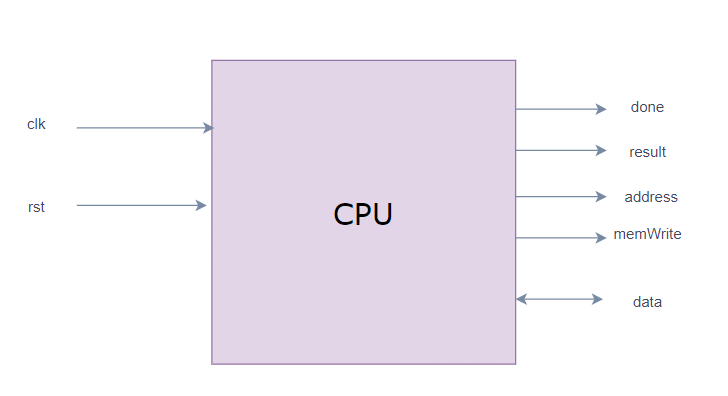
\includegraphics[width=\linewidth]{img/cpu_level_0}
%	\caption{\label{fig:label2} CPU Level 0 diagram}
%\end{figure}


%\begin{figure}[!htbp]
%	\centering
%	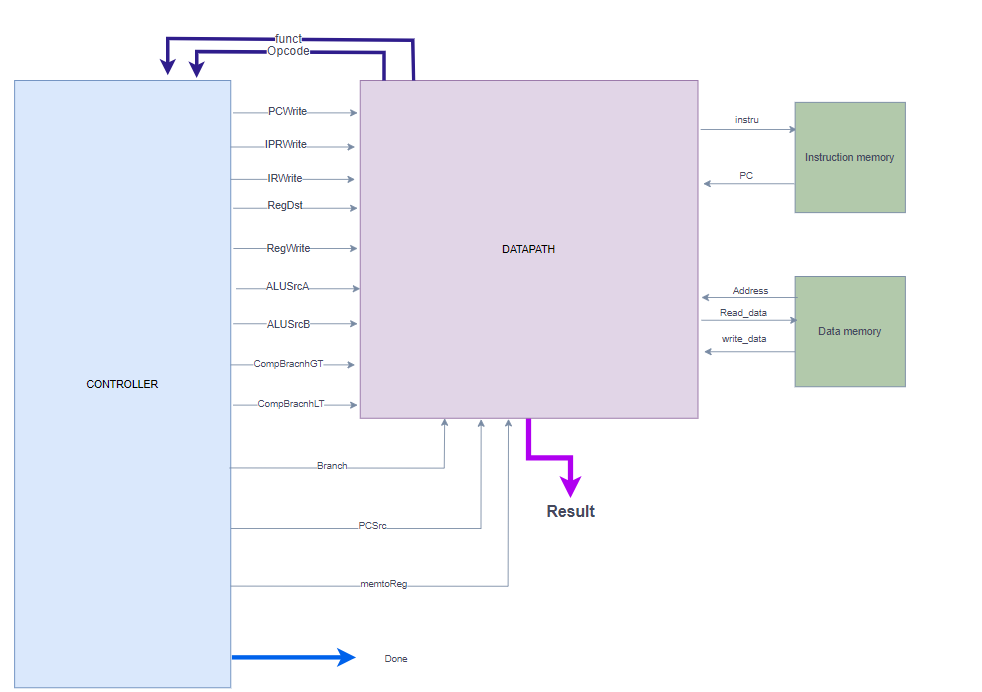
\includegraphics[width=\linewidth]{img/block_diagram}
%	\caption{\label{fig:label2} block diagram}
%\end{figure}

\section{CPU Level 1 diagram:}
\begin{figure}[!htbp]
	\centering
	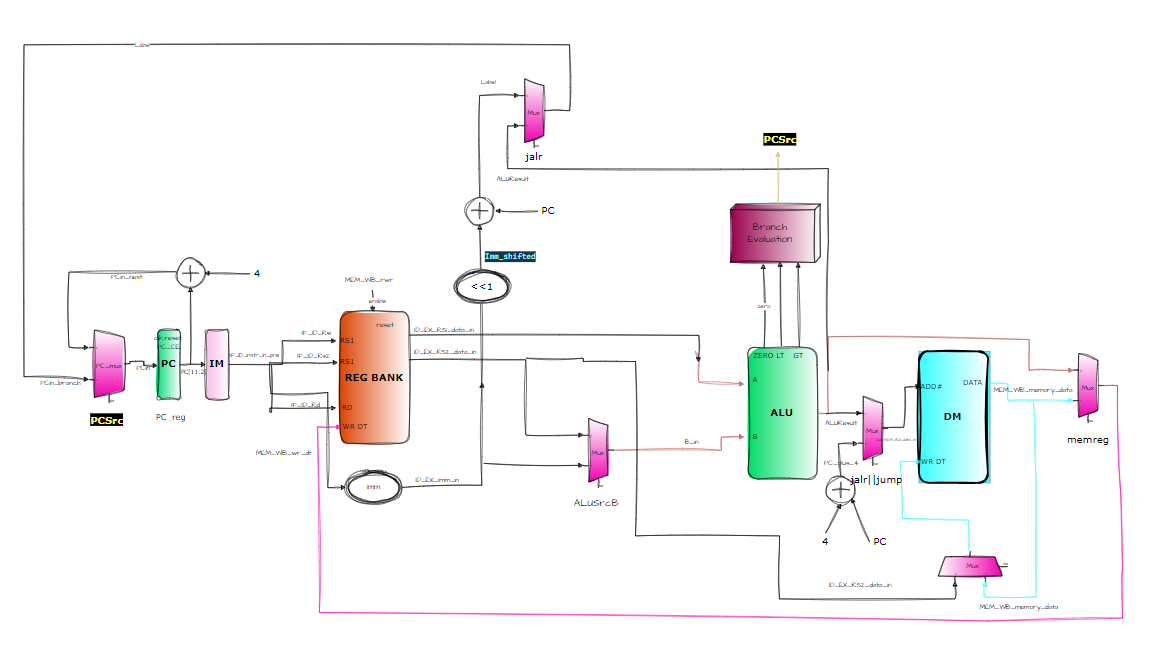
\includegraphics[width=\linewidth]{img/cpu_level_1}
	\caption{\label{fig:label2} block diagram}
\end{figure}


\subsection{Instruction Memory}

\noindent
\textbf{Program Counter (PC)} width = 32 bits \\
\textbf{Address width} = 32 bits \\
Bits 9 to 2 of the PC are used for pointing to the instructions. The lower 2 bits are not used so that the instructions are located at addresses which are multiples of 4. The address space is reduced for implementation purposes on the Basys 3 FPGA. \\
\textbf{Instruction width} = 32 bits \\
\textbf{Memory space} = 256 locations of 32 bits each. \\
This is realized using a distributed RAM implemented as a single port ROM in the FPGA.

\subsection{Register File}

\noindent
A set of 32 registers \(x_0\) to \(x_{31}\), each 32 bits wide. This register file has 2 asynchronous read ports and 1 synchronous write port. Register \(x_0\) always contains the value 0.
\subsection{Immediate Generation Unit}

\noindent
A module that takes in the instruction, extracts the 12-bit immediate/offset field from it, and sign extends it to 32 bits. The Most Significant Bit (MSB) is sign extended to all the upper positions in the output.


\subsection{Controller}
\subsection*{Control Signal Purposes}

\noindent
The following table describes the purposes of various control signals:

\begin{table}[h!]
	\centering
	\resizebox{\textwidth}{!}{%
		\begin{tabular}{|c|c|}
			\hline
			\textbf{Control Signal} & \textbf{Purpose} \\
			\hline
			ALUOp[1:0] & Tells the ALU Decoder what control signal to generate/what field to look at to figure out which control signal to generate. \\
			\hline
			ASrc & Selects the first operand to be fed into the ALU, either the PC or register data. \\
			\hline
			ALUSrc & Selects the second operand to be passed on to the ALU, either register data or sign-extended immediate. \\
			\hline
			BSrc & Selects the second operand to be fed into the ALU, either the value passed by the ALUMux or 4. \\
			\hline
			memreg & Selects the data to be written to the register bank, i.e., either data from memory or computed result from ALU. \\
			\hline
			dmr & Enables the data memory to be read from. \\
			\hline
			dmw & Enables the data memory to be written to. \\
			\hline
			rwr & Enables write to happen to the register file. \\
			\hline
			jalr & Selects the data to be written to the register file in case of JALR instruction, i.e., selects PC+4. Also selects the appropriate branch target address in case of JALR instruction. \\
			\hline
			Branch & Asserted for branch type of instructions. Enables updating of PC with branch target address. \\
			\hline
			Jump & Asserted for jump type of instructions. Enables updating of PC with target address. \\
			\hline
			Halt & Asserted when HALT instruction is encountered. Disables further instructions filling into the pipeline. \\
			\hline
			lw, lh, lhu, lb, lbu & Generated when LOAD type instruction is encountered. Specify with what data the destination register has to be loaded, i.e., byte/half-word/word. \\
			\hline
			sw, sh, sb & Generated when STORE type instruction is encountered. Specify with what data the destination memory address has to be written with, i.e., byte/half-word/word. \\
			\hline
			PCSrc & Selects the result with which the PC needs to be updated, i.e., either the address of the next instruction (PC+4) or branch target address. \\
			\hline
		\end{tabular}%
	}
	\caption{Control Signal Purposes}
\end{table}


\section{ALU Decoder and ALU}

\subsection{ALU}

The ALU is a 16-bit unit that supports the following instructions:
\begin{itemize}
	\item ADD
	\item SUB
	\item AND
	\item OR
	\item XOR
	\item NOT
	\item LSL (Logical Shift Left)
	\item LSR (Logical Shift Right)
	\item ASR (Arithmetic Shift Right)
\end{itemize}

In addition to the result, the ALU generates the following flags:
\begin{itemize}
	\item Greater Than or Equal To (GE)
	\item Less Than (LT)
	\item Zero (Z)
\end{itemize}

\subsection{ALU Decoder and Control}

The control unit has two decoders:
\begin{enumerate}
	\item \textbf{Main Decoder:} This decoder takes the opcode and issues the appropriate \texttt{ALUOp[1:0]} signal to the ALU decoder.
	\item \textbf{ALU Decoder:} Based on the function field and \texttt{ALUOp} signal, the ALU decoder generates the \texttt{ALUControl[3:0]} signal.
\end{enumerate}

\noindent
\texttt{ALUOp} is generated as follows:
\begin{itemize}
	\item For arithmetic operations, \texttt{ALUOp} may specify the need for addition or subtraction.
	\item For logical operations, \texttt{ALUOp} helps in selecting operations like AND, OR, XOR.
	\item For shift operations, \texttt{ALUOp} will determine if a shift left or shift right is performed.
\end{itemize}
ALUOp is generated as
\begin{table}[ht]
	\centering
	\begin{tabular}{|c|c|c|}
		\hline
		\textbf{Instruction} & \textbf{ALUOp} & \textbf{Operation} \\
		\hline
		R-type & 10 & Look at func3/func7 \\
		\hline
		I-type & 00 & ADD \\
		\hline
		Loads & 00 & ADD \\
		\hline
		Stores & 00 & ADD \\
		\hline
		Branches & 01 & Look at func3 \\
			\hline
		LUI & 11 & Look at func3 \\
		\hline
		JAL & 00 & ADD \\
		\hline
		JALR & 00 & ADD \\
		\hline
		NOP & 11 & Other/Do nothing \\
		\hline
		HALT & 11 & Other/Do nothing \\
		\hline
	\end{tabular}
	\caption{ALUOp and Corresponding Operations}
	\label{tab:aluop_operations}
\end{table}

ALUControl is generated as 
\begin{table}[ht]
	\centering
	\begin{tabular}{|c|c|c|}
		\hline
		\textbf{Instruction} & \textbf{Func 3/Func 7} & \textbf{ALUControl} \\
		\hline
		ADD & 000/0000000 & 0010 \\
		\hline
		SUB & 000/0100000 & 0110 \\
		\hline
		AND & 111 & 0000 \\
		\hline
		OR  & 110 & 0001 \\
		\hline
		XOR & 100 & 0011 \\
		\hline
		SLL & 001 & 0100 \\
		\hline
		SRL & 101/0000000 & 0101 \\
		\hline
		SRA & 101/0100000 & 0111 \\
		\hline
		NOP & 000/0000000 & 1010 \\
		\hline
		HALT & 000/0000000 & 1010 \\
		\hline
	\end{tabular}
	\caption{ALUControl Values for R-Type Instructions}
	\label{tab:alucontrol_rtype}
\end{table}


\begin{table}[ht]
	\centering
	\begin{tabular}{|c|c|c|}
		\hline
		\textbf{Instruction} & \textbf{Func 3} & \textbf{ALUControl} \\
		\hline
		BEQ & 000 & 0110 \\
		\hline
		BNE & 001 & 0110 \\
		\hline
		BLT & 100 & 1000 \\
		\hline
		BGE & 101 & 1001 \\
		\hline
	\end{tabular}
	\caption{ALUControl Values for Branch Instructions}
	\label{tab:alucontrol_branches}
\end{table}
For all other instructions, ALUControl = 0010 (ADD)


%\begin{figure}[!htbp]
%	\centering
%	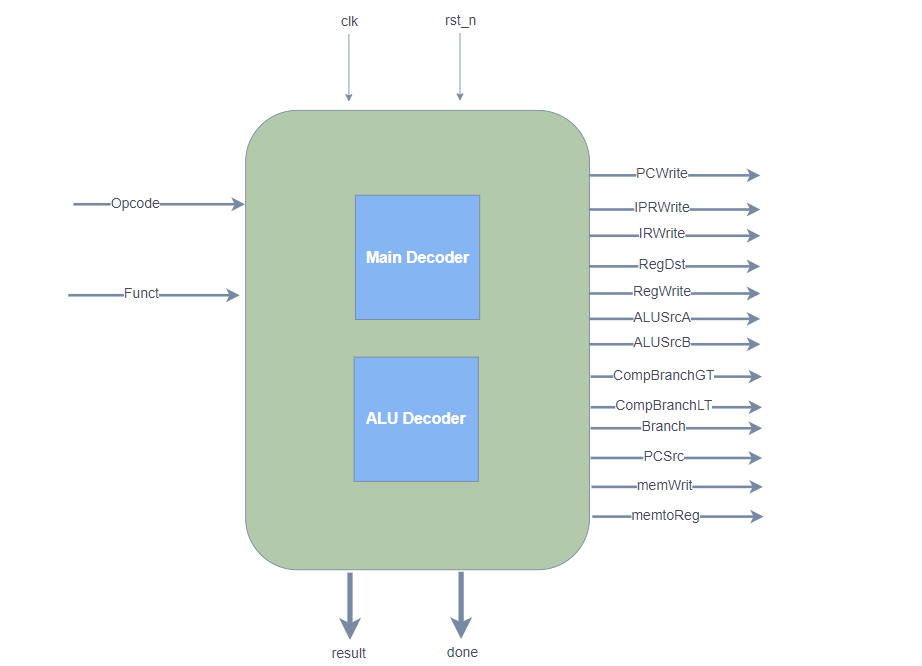
\includegraphics[width=\linewidth]{img/decoder}
%	\caption{\label{fig:label2} CPU Level 1 diagram}
%\end{figure}



%\subsection{Pseudo code}
%\begin{algorithm}
%	\caption{System Initialization, Configuration, and Main Loop}
%	\begin{algorithmic}
%		\STATE \textbf{Initialization and Configuration}
%		\STATE Initialize the system clock
%		\STATE Configure UART:
%		\STATE \ \ \ \ Enable UART0 and GPIOA peripherals
%		\STATE \ \ \ \ Set up UART pins PA0 and PA1
%		\STATE \ \ \ \ Configure UART settings (baud rate, data format)
%		\STATE \ \ \ \ Enable UART interrupts
%		
%		\STATE Configure SysTick Timer:
%		\STATE \ \ \ \ Disable SysTick Timer
%		\STATE \ \ \ \ Set reload value for 20ms period
%		\STATE \ \ \ \ Enable SysTick Timer and interrupts
%		
%		\STATE Configure ADC:
%		\STATE \ \ \ \ Enable GPIOE and ADC0 peripherals
%		\STATE \ \ \ \ Set up GPIOE for analog input
%		\STATE \ \ \ \ Configure ADC0 settings and enable sequencer 3
%		
%		\STATE Configure PWM:
%		\STATE \ \ \ \ Enable PWM0 module and configure PWM output
%		\STATE \ \ \ \ Set initial PWM settings and direction
%		
%		\STATE Enable global interrupts
%		
%		\STATE \textbf{Main Loop}
%		\WHILE {true}
%		\STATE Delay for 1ms
%		\STATE Calculate RPM based on QEI speed
%		\STATE Print direction, theta, RPM, and ADC readings to UART
%		\ENDWHILE
%		
%		\STATE \textbf{SysTick Handler}
%		\STATE If PWM compare value is above threshold:
%		\STATE \ \ \ \ Set direction to 1
%		\STATE Else:
%		\STATE \ \ \ \ Set direction to 0
%		\STATE \ \ \ \ Toggle GPIO pins
%		\STATE Adjust PWM compare value based on direction
%		
%		\STATE \textbf{Function Definitions}
%		\STATE \textbf{Function \texttt{uart\_print\_num(x)}}
%		\IF {x is negative}
%		\STATE Print '-' character
%		\STATE Convert x to positive
%		\ENDIF
%		\STATE Convert x to a string
%		\STATE Print each digit of x to UART
%		
%		\STATE \textbf{Function \texttt{get\_adc\_value(channel)}}
%		\STATE Set ADC channel
%		\STATE Start ADC conversion
%		\STATE Wait for conversion to complete
%		\STATE Read ADC result and average over 32 samples
%		\STATE Convert result to millivolts
%		\STATE Return ADC value in millivolts
%		
%		\STATE \textbf{Function \texttt{delayMs(n)}}
%		\STATE Create a delay of n milliseconds by looping
%		
%	\end{algorithmic}
%\end{algorithm}
%\section{Controller FSM:}
%\begin{figure}[!htbp]
%	\centering
%	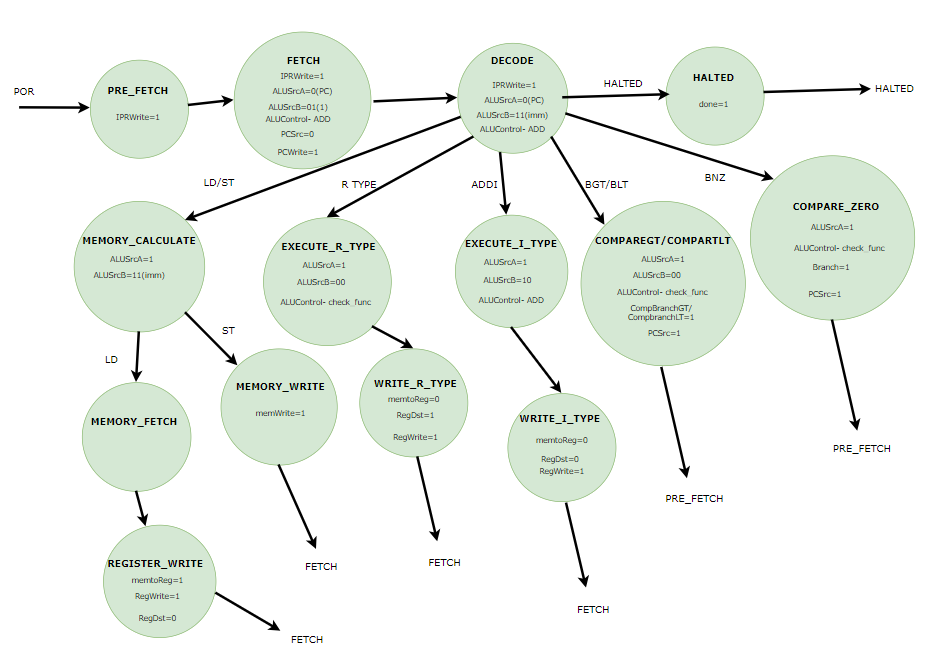
\includegraphics[width=\linewidth]{img/fsm}
%	\caption{\label{fig:final_setup}FSM}
%\end{figure}

\section{Data memory and load and store hardware}
\noindent
The data memory is implemented using a distributed RAM  with the following specifications:

\begin{itemize}
	\item \textbf{Write Width}: 32 bits
	\item \textbf{Write Depth}: 1024 locations
	\item \textbf{Byte Writable}: The memory locations are byte-writable.
	\item \textbf{Read and Write Access}: Both reads and writes are synchronous operations.
%	\item \textbf{Latency}: 1 clock cycle
\end{itemize}
\noindent
The store hardware generates appropriate write enable signals for the data memory based on the control signals `sw`, `sh`, and `sb`. The write enable signals are determined as follows:

\begin{itemize}
	\item \textbf{`sw` (Store Word)}: 
	\begin{itemize}
		\item Generates a write enable signal for the entire 32-bit word.
		\item Writes the 32-bit value to the specified memory location.
	\end{itemize}
	
	\item \textbf{`sh` (Store Half-word)}:
	\begin{itemize}
		\item Generates write enable signals for two contiguous 16-bit half-words.
		\item Writes the lower 16 bits to the lower address and the upper 16 bits to the higher address if the memory is byte-addressable.
	\end{itemize}
	
	\item \textbf{`sb` (Store Byte)}:
	\begin{itemize}
		\item Generates a write enable signal for a single byte in the 32-bit word.
		\item Writes the byte to the specified byte-addressable location.
	\end{itemize}
\end{itemize}

\noindent
The control signals `sw`, `sh`, and `sb` select the appropriate write enable signals, ensuring the correct data is written to the memory based on the type of store operation.
\begin{figure}[!htbp]
	\centering
	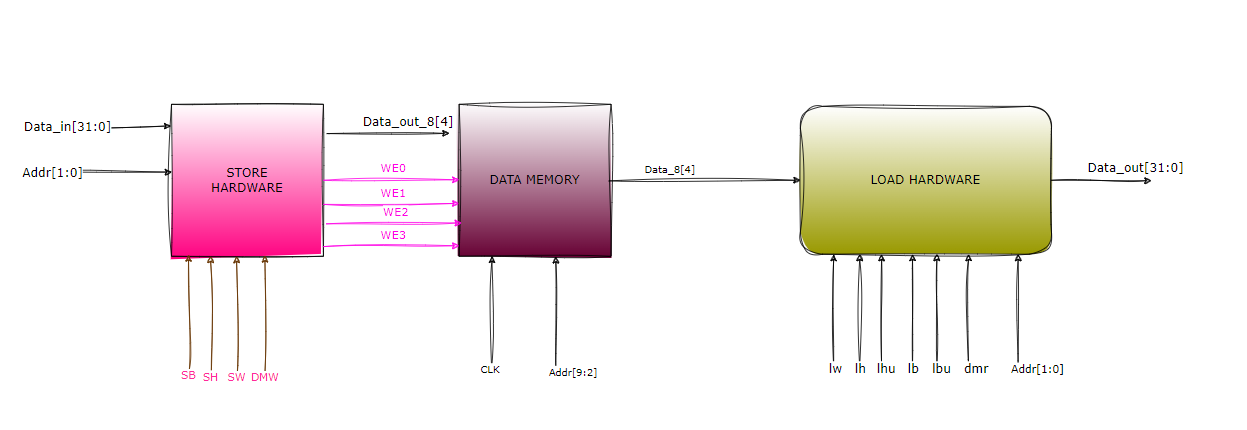
\includegraphics[width=\linewidth]{img/storage}
	\caption{\label{fig:storage}storage circuit logic}
\end{figure}
\begin{tabular}{|c|c|c|c|c|c|c|c|c|c|}
	\hline
	Instruction & A1 & A0 & sw & sh & sb & WE0 & WE1 & WE2 & WE3 \\
	\hline
	SW & 0 & 0 & 1 & 0 & 0 & 1 & 1 & 1 & 1 \\
	\hline
	SH & 0 & 0 & 0 & 1 & 0 & 1 & 1 & 0 & 0 \\
	\hline
	SH & 1 & 0 & 0 & 1 & 0 & 0 & 0 & 1 & 1 \\
	\hline
	SB & 0 & 0 & 0 & 0 & 1 & 1 & 0 & 0 & 0 \\
	\hline
	SB & 0 & 1 & 0 & 0 & 1 & 0 & 1 & 0 & 0 \\
	\hline
	SB & 1 & 0 & 0 & 0 & 1 & 0 & 0 & 1 & 0 \\
	\hline
	SB & 1 & 1 & 0 & 0 & 1 & 0 & 0 & 0 & 1 \\
	\hline
\end{tabular}

\subsection{Load Hardware}

\noindent
The load hardware is situated in the Write-Back (WB) stage of the pipeline, as opposed to the MEM stage used for store hardware. This positioning is due to the synchronous read nature of the Distributed RAM  used in the implementation. Consequently, all control signals for load operations are delayed until the WB stage.

\noindent
In the WB stage, the load hardware is responsible for constructing the appropriate 32-bit word to be loaded into the CPU register. This construction is based on the control signals received, which determine the specific operation to be performed. The load hardware ensures that the data read from memory is correctly formatted and transferred to the register file, completing the data retrieval process.

%\begin{figure}[h!]
%	\centering
%	\includegraphics[width=\textwidth]{load_hardware_diagram} % Replace with your diagram
%	\caption{Load Hardware Block Diagram}
%\end{figure}

\noindent
The control signals used for load operations include those that determine the type of load instruction (e.g., byte, half-word, word) and manage the data path to ensure proper data retrieval and storage.

\noindent
The following table summarizes the control signals and data formatting for various load instructions. The `Data` field represents the data read from memory, with different bit widths and sign extension applied based on the instruction.
\\
\begin{longtable}{|c|c|c|c|c|c|c|c|c|}
	\hline
	\textbf{Instruction} & \textbf{A1} & \textbf{A0} & \textbf{LW} & \textbf{LH} & \textbf{LHU} & \textbf{LB} & \textbf{LBU} & \textbf{Data to Register} \\
	\hline
	\endfirsthead
	\hline
	\textbf{Instruction} & \textbf{A1} & \textbf{A0} & \textbf{LW} & \textbf{LH} & \textbf{LHU} & \textbf{LB} & \textbf{LBU} & \textbf{Data to Register} \\
	\hline
	\endhead
	\hline
	\endfoot
	\hline
	\endlastfoot
	\hline
	LW  & 0 & 0 & 1 & 0 & 0 & 0 & 0 & Data[31:0] \\
	\hline
	LH  & 0 & 0 & 0 & 1 & 0 & 0 & 0 & \{16\{Data[15], Data[15:0]\} \\
\hline
LH  & 0 & 1 & 0 & 1 & 0 & 0 & 0 & \{16\{Data[31], Data[31:16]\} \\
\hline
LHU & 0 & 0 & 0 & 0 & 1 & 0 & 0 & \{16\{0\}, Data[15:0]\} \\
\hline
LHU & 0 & 1 & 0 & 0 & 1 & 0 & 0 & \{16\{0\}, Data[31:16]\} \\
\hline
LB  & 0 & 0 & 0 & 0 & 0 & 1 & 0 & \{24\{Data[7], Data[7:0]\} \\
\hline
LB  & 0 & 1 & 0 & 0 & 0 & 1 & 0 & \{24\{Data[15], Data[15:8]\} \\
\hline
LB  & 1 & 0 & 0 & 0 & 0 & 1 & 0 & \{24\{Data[23], Data[23:16]\} \\
\hline
LB  & 1 & 1 & 0 & 0 & 0 & 1 & 0 & \{24\{Data[31], Data[31:24]\} \\
\hline
LBU & 0 & 0 & 0 & 0 & 0 & 0 & 1 & \{24\{0\}, Data[7:0]\} \\
\hline
LBU & 0 & 1 & 0 & 0 & 0 & 0 & 1 & \{24\{0\}, Data[15:8]\} \\
\hline
LBU & 1 & 0 & 0 & 0 & 0 & 0 & 1 & \{24\{0\}, Data[23:16]\} \\
\hline
LBU & 1 & 1 & 0 & 0 & 0 & 0 & 1 & \{24\{0\}, Data[31:24]\} \\
\hline
\end{longtable}


%\begin{tikzpicture}[node distance=2cm]
%	
%	% Nodes
%	\node (start) [startstop] {Start};
%	\node (dmr) [decision, below of=start, yshift=-1cm] {Is dmr asserted?};
%	\node (lw) [decision, below of=dmr, yshift=-1cm] {Is lw asserted?};
%	\node (load32) [process, below of=lw, yshift=-1cm] {Load 32-bit word};
%	\node (lh_lhu) [decision, right of=lw, xshift=4cm] {Is lh or lhu asserted?};
%	\node (lh) [decision, below of=lh_lhu] {Is lh asserted?};
%	\node (addr1_lh) [decision, below of=lh, yshift=-1cm] {Is addr[1] set (lh)?};
%	\node (load_upper_lh) [process, below of=addr1_lh, yshift=-1cm] {Load upper 16-bit with sign-extension};
%	\node (load_lower_lh) [process, right of=load_upper_lh, xshift=4cm] {Load lower 16-bit with sign-extension};
%	\node (addr1_lhu) [decision, below of=lh_lhu, yshift=-1cm] {Is addr[1] set (lhu)?};
%	\node (load_upper_lhu) [process, below of=addr1_lhu, yshift=-1cm] {Load upper 16-bit without sign-extension};
%	\node (load_lower_lhu) [process, right of=load_upper_lhu, xshift=4cm] {Load lower 16-bit without sign-extension};
%	\node (lb_lbu) [decision, right of=lh_lhu, xshift=4cm] {Is lb or lbu asserted?};
%	\node (lbu) [decision, below of=lb_lbu] {Is lbu asserted?};
%	\node (load_byte_lbu) [process, below of=lbu] {Load byte without sign-extension};
%	\node (load_byte_lb) [process, right of=load_byte_lbu, xshift=4cm] {Load byte with sign-extension};
%	\node (data0) [process, below of=lb_lbu, yshift=-3cm] {data\_out = 32'd0};
%	
%	\node (end) [startstop, below of=data0, yshift=-1cm] {End};
%	
%	% Arrows
%	\draw [arrow] (start) -- (dmr);
%	\draw [arrow] (dmr) -- node[anchor=east] {Yes} (lw);
%	\draw [arrow] (lw) -- node[anchor=east] {Yes} (load32);
%	\draw [arrow] (load32) -- (data0);
%	\draw [arrow] (dmr) -- node[anchor=west] {No} (data0);
%	\draw [arrow] (lw) -- node[anchor=north] {No} (lh_lhu);
%	\draw [arrow] (lh_lhu) -- node[anchor=east] {Yes} (lh);
%	\draw [arrow] (lh) -- node[anchor=east] {Yes} (addr1_lh);
%	\draw [arrow] (addr1_lh) -- node[anchor=east] {Yes} (load_upper_lh);
%	\draw [arrow] (addr1_lh) -- node[anchor=south] {No} (load_lower_lh);
%	\draw [arrow] (lh) -- node[anchor=north] {No} (addr1_lhu);
%	\draw [arrow] (addr1_lhu) -- node[anchor=east] {Yes} (load_upper_lhu);
%	\draw [arrow] (addr1_lhu) -- node[anchor=south] {No} (load_lower_lhu);
%	\draw [arrow] (lh_lhu) -- node[anchor=north] {No} (lb_lbu);
%	\draw [arrow] (lb_lbu) -- node[anchor=east] {Yes} (lbu);
%	\draw [arrow] (lbu) -- node[anchor=east] {Yes} (load_byte_lbu);
%	\draw [arrow] (lbu) -- node[anchor=south] {No} (load_byte_lb);
%	\draw [arrow] (lb_lbu) -- node[anchor=west] {No} (data0);
%	\draw [arrow] (data0) -- (end);
%	
%\end{tikzpicture}

\section{Forwarding Unit}


\noindent
The forwarding unit generates appropriate control signals to forward data from subsequent stages to the input of the EX/MEM stages in case of a data hazard.

\noindent
\textbf{FA/FB Forwarding} control signals are as follows:

\begin{longtable}{|c|c|}
	\hline
	\textbf{FA/FB } & \textbf{Description} \\
	\hline
	\endfirsthead
	\hline
	\textbf{FA/FB } & \textbf{Description} \\
	\hline
	\endhead
	\hline
	\endfoot
	\hline
	\endlastfoot
	\hline
	00 & Input taken from IF\_ID pipeline register (No forwarding) \\
	\hline
	01 & Input taken from WB\_FIN pipeline register \\
	\hline
	10 & Input taken from MEM\_WB pipeline register \\
	\hline
	11 & Input taken from EX\_MEM pipeline register \\
	\hline
\end{longtable}

\noindent
In the case where a load is followed by a store instruction, where \texttt{STORE.Rs2} = \texttt{LOAD.Rd}, forwarding needs to be done from the MEM\_WB pipeline register to the write data port of the data memory. The control signal \texttt{FS} facilitates this.
\section{Stalling and Halting Unit}

\noindent
The stalling and halting unit generates appropriate control signals to stall or halt execution.

\noindent
In case of a LOAD instruction followed by a dependent instruction, only forwarding will not suffice. A 1-stall cycle needs to be introduced.

\noindent
In case the branching condition is satisfied, 1 stall cycle and 1 NOP instruction need to be introduced into the pipeline.

\noindent
The following table summarizes the conditions for stalling and halting, with the associated control signals.

\begin{longtable}{|c|c|c|p{5cm}|c|c|c|c|c|}
	\hline
	\textbf{Hazard} & \textbf{PCSrc} & \textbf{Halt} & \textbf{dmr \&\& ((IF/ID.RS1==ID/EX.Rd) or (IF/ID.RS2==ID/EX.Rd))} & \textbf{Stall} & \textbf{Discont} & \textbf{PC\_CE} & \textbf{IF\_ID\_CE} \\
	\hline
	Data & 0 & 0 & 1 & 0 & 1 & 0 & 0 \\
	\hline
	Control & 1 & 0 & 0 & 1 & 1 & 1 & 1 \\
	\hline
	- & 0 & 1 & 0 & 0 & 0 & 1 & 1 \\
	\hline
\end{longtable}


\section{Instruction Cache}

\subsection*{Blocks and Specifications:}

\begin{enumerate}
	\item \textbf{Instruction Memory (Block RAM)}
	\begin{itemize}
		\item Size: 256 words (1 kB)
		\item Address bits: \( \log_2 256 = 8 \)
		\item Since addresses are multiples of 4, the 2 least significant bits of the PC are always 0.
		\item PC[9:2] are used to index into the main memory.
	\end{itemize}
	
	\item \textbf{Instruction Cache Memory}
	\begin{itemize}
		\item Size: 32 words
		\item Associativity: 2-way set associative
		\item Block/line size: 4 words
		\item Number of lines: \( \frac{32}{4} = 8 \)
		\item Number of sets: \( \frac{8}{2} = 4 \)
	\end{itemize}
	
	\item \textbf{Instruction Tag RAM}
	\begin{itemize}
		\item Locations: 8 (same as the number of lines)
		\item Each line contains used, valid, and tag bits:
		\begin{itemize}
			\item USED (1 bit)
			\item VALID (1 bit)
			\item TAG (4 bits)
		\end{itemize}
	\end{itemize}
	
	\item \textbf{Cache Controller}
	\begin{itemize}
		\item Issues control signals to manage cache hits and misses.
	\end{itemize}
	
	\item \textbf{Shift Register}
	\begin{itemize}
		\item Size: 4 words (128 bits)
		\item Words are shifted into this register one at a time until the entire line is filled.
	\end{itemize}
	
	\item \textbf{Counter Block}
	\begin{itemize}
		\item Size: 3 bits (8 counts)
		\item Counts cycles and issues control signals to the cache controller to update the cache in a fixed number of cycles.
	\end{itemize}
	
	\item \textbf{Hit Circuitry}
	\begin{itemize}
		\item Determines if an instruction is a hit or miss:
		\begin{itemize}
			\item If \((\text{tag}_0 = \text{tag} \text{ and } v_0 = 1)\) then \textbf{Hit}
			\item Else if \((\text{tag}_1 = \text{tag} \text{ and } v_1 = 1)\) then \textbf{Hit}
			\item Else \textbf{Miss}
		\end{itemize}
	\end{itemize}
	
	\item \textbf{Word MUX}
	\begin{itemize}
		\item Selects the required word from the 4 words in the cache line based on PC[3:2].
	\end{itemize}
\end{enumerate}

\noindent The physical address is split as follows:

%\begin{center}
%	\begin{tabular}{|c|c|c|c|c|c|c|c|c|c|}
%		\hline
%		7 & \multicolumn{3}{c|}{\textbf{TAG}} & 3 & \multicolumn{2}{c|}{\textbf{SET}} & 2 & 1 & \textbf{Block Offset} \\
%		\hline
%	\end{tabular}
%\end{center}
\noindent \texttt{7 [TAG] 4 || 3 [SET] 2 || 1 [Block offset] 0}
%\begin{table}[h!]
%	\centering
%	\begin{tabular}{|c|c|c|c|c|c|c|c|c|c|}
%		\hline
%		\textcolor{blue}{7} & \multicolumn{3}{c|}{\textbf{TAG}} & \textcolor{blue}{4} & \textcolor{blue}{3} & \textbf{SET} & \textcolor{blue}{2} & \textcolor{blue}{1} & \textbf{Block offset} \textcolor{blue}{0} \\
%		\hline
%	\end{tabular}
%\end{table}

\begin{figure}[!htbp]
	\centering
	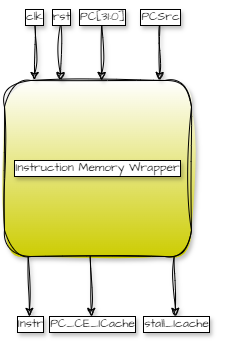
\includegraphics[height=0.4\linewidth,width=0.4\linewidth]{img/instru_cache}
	\caption{\label{fig:instru_cache} Level 0 of Instruction cache}
\end{figure}

\subsection{Instruction Cache Controller FSM}

\begin{itemize}
	\item \textbf{TAG COMPARE}: The incoming address is decomposed into a set number and a tag. The set number indexes both banks of the instruction cache memory and both banks of the instruction tag RAM. A cache hit occurs if the tags match and the cache line is valid; otherwise, it results in a miss. In this state, it is determined if there is a cache miss or hit.
	
	\item \textbf{READ IMEM}: This state prepares the FSM to read the missed line from the instruction memory in a fixed number of clock cycles by resetting the counter.
	
	\item \textbf{WAIT IMEM}: The missed line is read from the instruction memory word by word over 4 clock cycles. In this state, the controller waits for the memory operation to complete and for the instruction to be available at the cache input.
	
	\item \textbf{UPDATE CACHE}: The control signals required to write to the cache are set in this state. These control signals are configured based on which cache line is to be updated.
\end{itemize}
\subsection{Cache Controller Outputs}

\begin{itemize}
	\item \textbf{PC\_CE\_Icache}: When deasserted, it disables the PC from incrementing, allowing the processor to wait until the required instruction is brought into the cache.
	
	\item \textbf{Stall\_Icache}: When asserted, this signal introduces NOP instructions into the Decode stage, ensuring that no operation is performed until the required instruction is fetched into the cache.
	
	\item \textbf{Imem\_rd}: Connected to the enable pin of the Block RAM (BRAM). When asserted, data can be read from the BRAM.
	
	\item \textbf{next\_u0, next\_u1}: These are the updated values of the "used" bits for both lines in the selected set. They are written to the Instruction Tag RAM whenever a cache line is updated.
	
	\item \textbf{next\_v0, next\_v1}: These are the updated values of the "valid" bits for both lines in the selected set. They are written to the Instruction Tag RAM whenever a cache line is updated.
	
	\item \textbf{we\_t0, we\_t1}: These signals are asserted to enable writing to the Instruction Tag RAM. Both signals must be asserted on a cache miss.
	
	\item \textbf{we\_I0, we\_I1}: These signals enable writing to the Instruction Cache memory. The specific signal corresponding to the line that needs to be updated within the set should be asserted.
	
	\item \textbf{next\_tag0, next\_tag1}: These are the updated values of the tag bits for the line to be updated in the selected set. They are written to the Instruction Tag RAM whenever a cache line is updated.
\end{itemize}
\begin{figure}[!htbp]
	\centering
	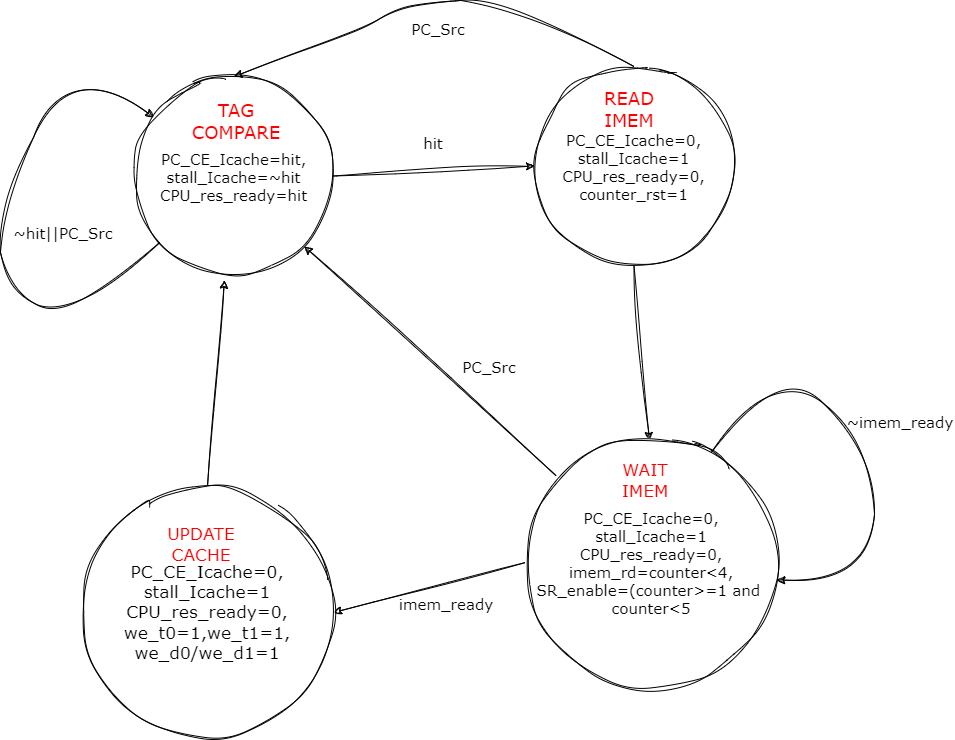
\includegraphics[width=\linewidth]{img/FSM_cache}
	\caption{\label{fig:FSM_cache} FSM of cache}
\end{figure}

\begin{figure}[!htbp]
	\centering
	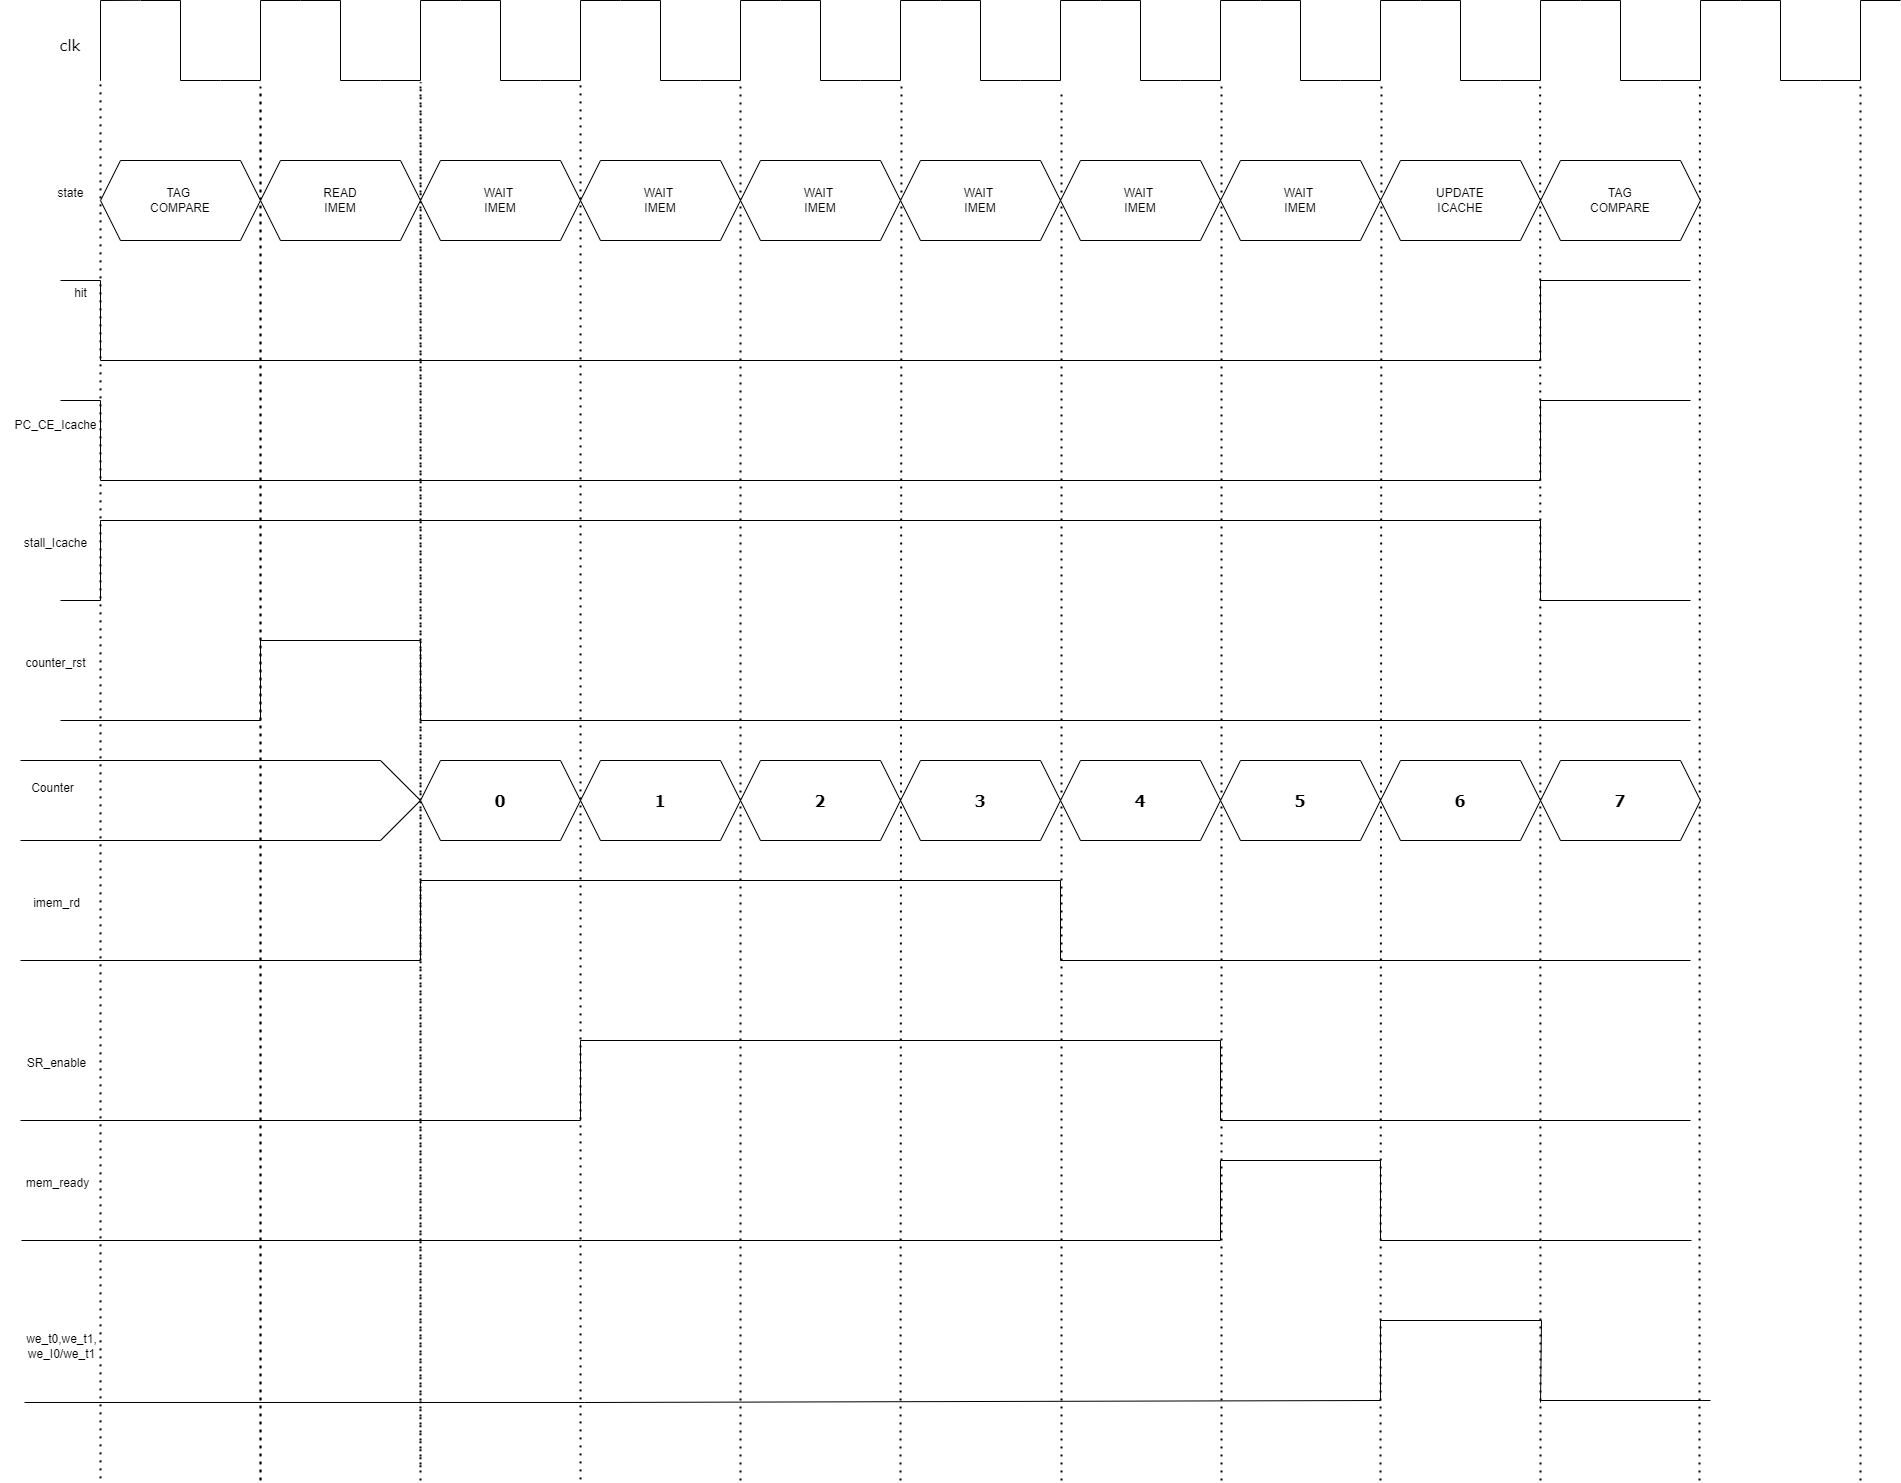
\includegraphics[width=\linewidth]{img/timing_cache}
	\caption{\label{fig:timing_cache} timing cache}
\end{figure}
\subsection{Rules for Cache Line Update}

\begin{enumerate}
	\item If neither line contains valid data, update line 0.
	\item If only one line contains valid data, update the line with invalid data.
	\item If both lines contain valid data, update the line that was least recently accessed. The "used" bit indicates recent access: $u = 0$ means the line was least recently used, while $u = 1$ means it was recently used.
\end{enumerate}

\subsection{Cache Operation Scenarios}

\textbf{Scenario 1: Instruction Hit}
\begin{enumerate}
	\item The set number and tag are extracted from the program counter (PC).
	\item The tags of both lines are compared with the extracted tag, and the valid bits are checked to determine if the lines have valid entries.
	\item If one of the lines contains the required instruction, the check results in a hit.
	\item The instruction is then passed through the stall multiplexer to the input of the IF/ID pipeline register.
\end{enumerate}

\textbf{Scenario 2: Instruction Miss}
\begin{enumerate}
	\item The set number and tag are extracted from the PC.
	\item The tags of both lines are compared with the extracted tag, and the valid bits are checked to determine if the lines have valid entries.
	\item If no line contains the required instruction, the check results in a miss. The $\text{PC\_CE\_Icache}$ signal is deasserted, and $\text{Stall\_Icache}$ is asserted.
	\item A NOP instruction is passed to the Decode and further stages. Meanwhile, the cache prepares to fetch the words from memory.
	\item The $\text{imem\_rd}$ signal is asserted, enabling the instruction word to be read. Over 4 consecutive cycles, 4 words (including the required word and three additional words to form a complete cache line) are shifted into a 128-bit shift register.
	\item After all 4 words are shifted in, the data becomes available at the cache input in the next cycle.
	\item The appropriate signals to write to the cache are asserted, allowing the data to be written at the next clock edge.
	\item The check from step 2 is repeated, resulting in a hit this time.
	\item The instruction is passed through the stall multiplexer to the input of the IF/ID pipeline register.
\end{enumerate}

\section{Testing:}
\begin{figure}[!htbp]
	\centering
	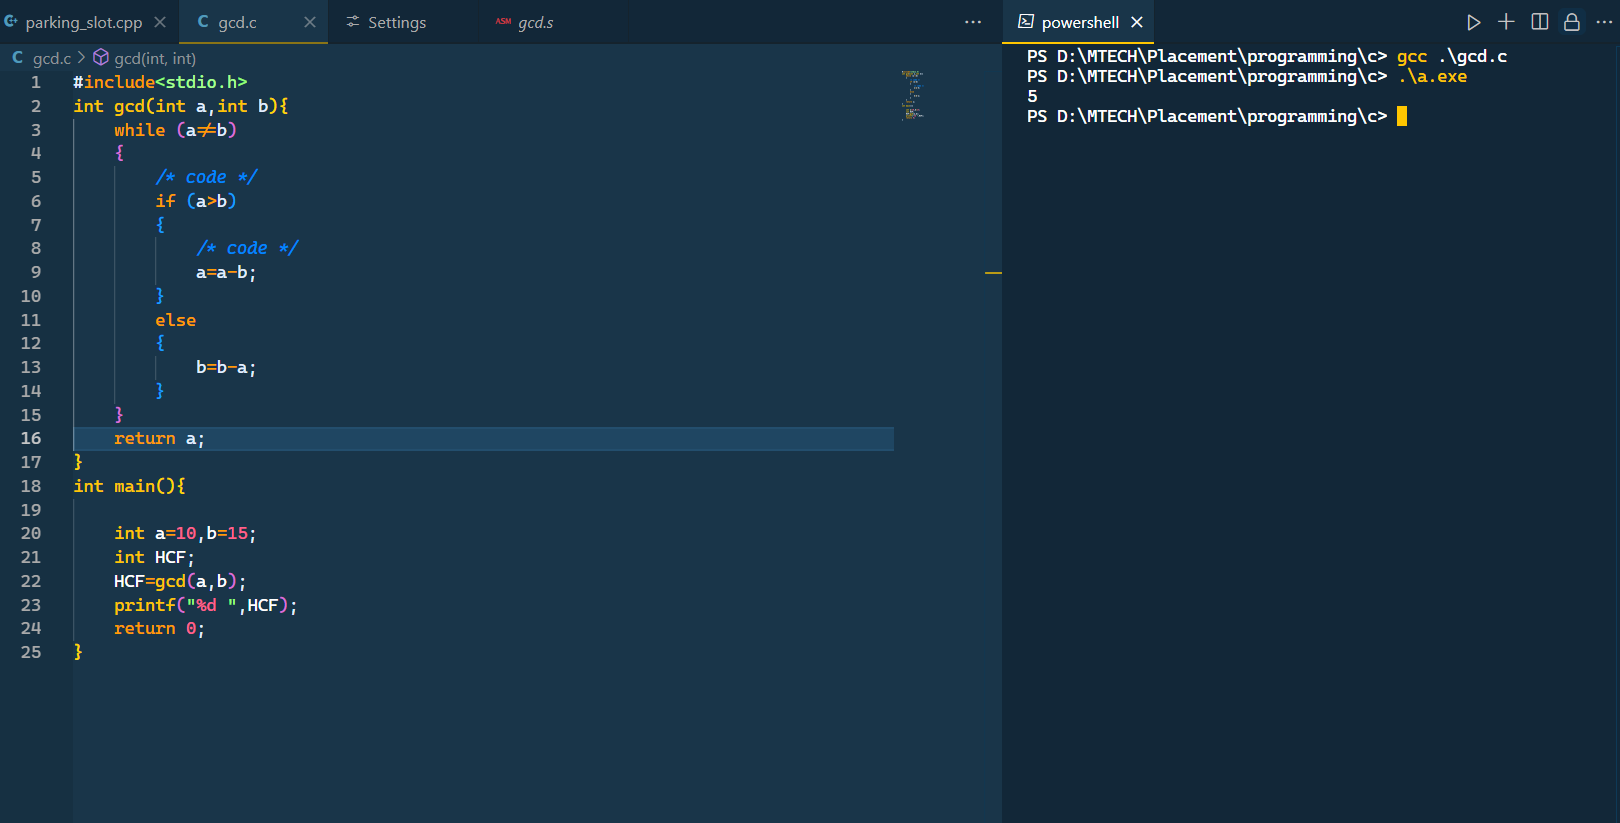
\includegraphics[width=\linewidth]{img/c_prog_gcd}
	\caption{\label{fig:c_prog_gcd} C prog of GCD}
\end{figure}

\begin{figure}[!htbp]
	\centering
	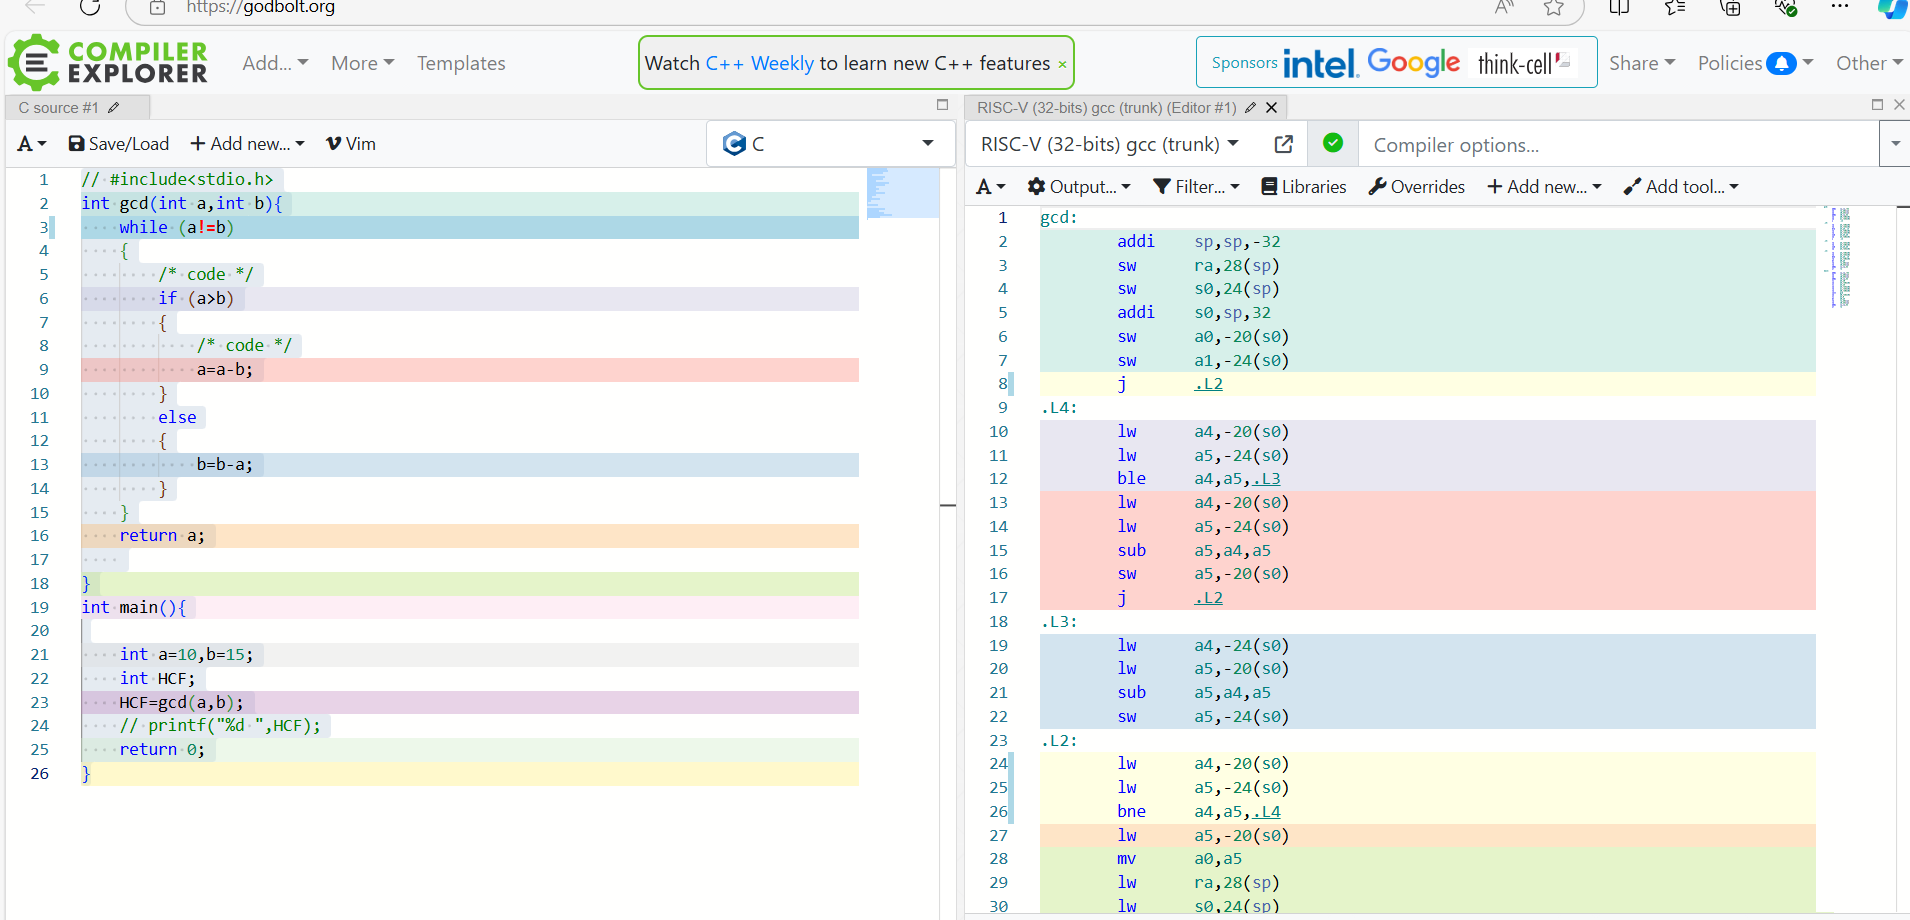
\includegraphics[width=\linewidth]{img/c_code_to_assembly_code}
	\caption{\label{fig:c_code_to_assembly_code} C code and assembly code conversion}
\end{figure}

\begin{figure}[!htbp]
	\centering
	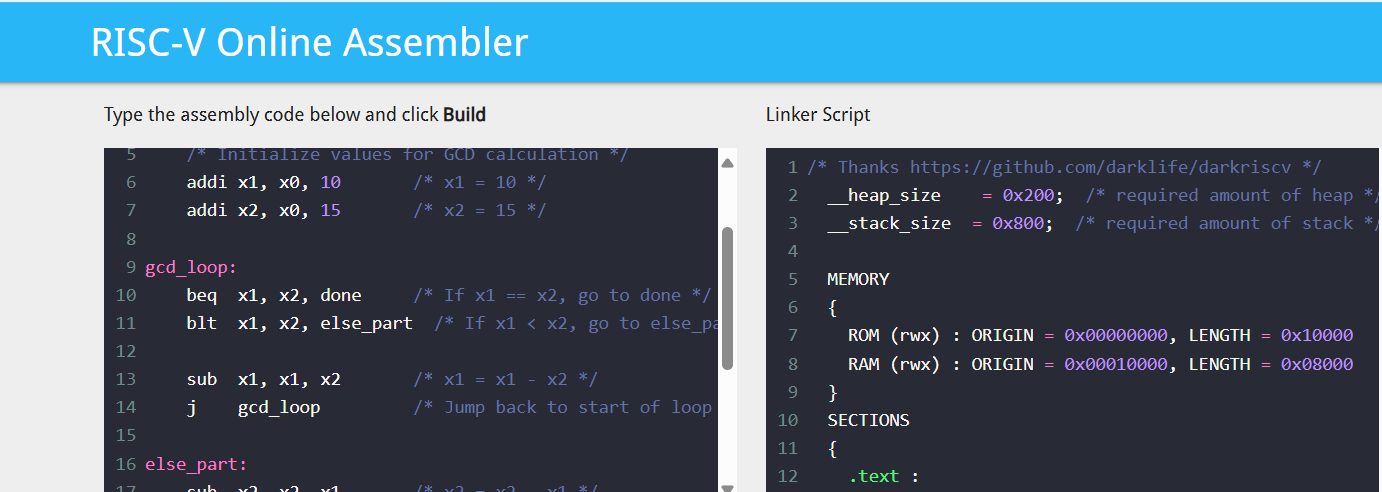
\includegraphics[width=\linewidth]{img/assembly_code_to_machine_code}
	\caption{\label{fig:assembly_code_to_machine_code}assembly code to machine code conversion}
\end{figure}





\begin{tabular}{|p{2cm}|p{3cm}|p{6cm}|p{4cm}|}
	\hline
	\textbf{PC} & \textbf{Label} & \textbf{Instruction} & \textbf{Machine Code} \\
	\hline
	0   &            & addi x1, x0, 10     & 00a00093 \\
	4   &            & addi x2, x0, 15     & 00f00113 \\
	8   & while\_loop& beq x1, x2, 24      & 00208C63 \\
	12  & if\_loop   & blt x1, x2, 12      & 0020C663 \\
	16  &            & sub x1, x1, x2      & 402080B3 \\
	20  &            & jal x0, -12         & ff5ff06f \\
	24  & else\_loop & sub x2, x2, x1      & 40110133 \\
	28  &            & jal x0, -20         & fedff06f \\
	32  &            & halt                & 0000001C \\
	\hline
\end{tabular}


\section{Results}

\subsection{RTL Schematic:}

\begin{figure}[!htbp]
	\centering
	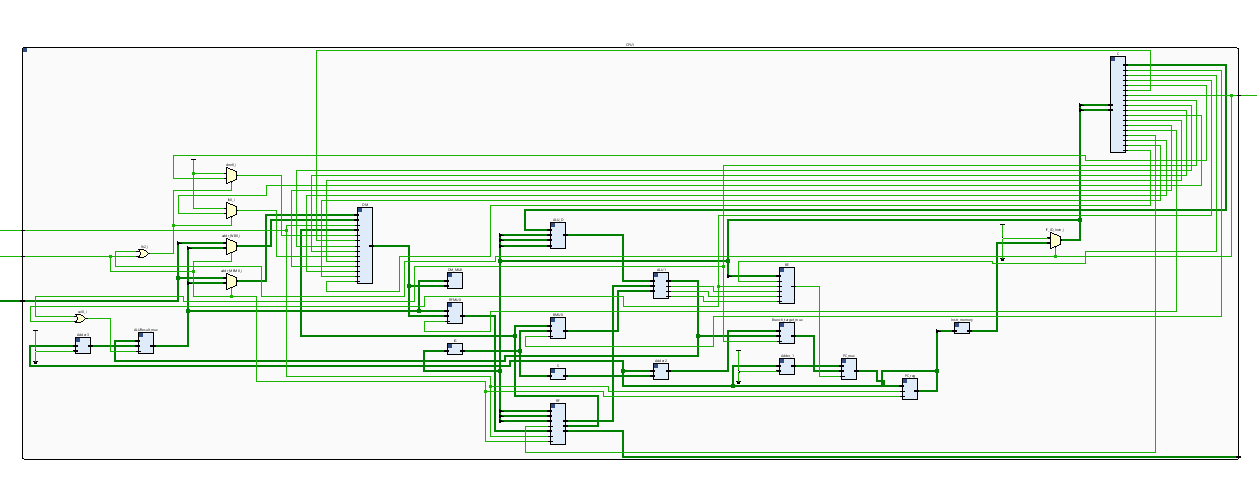
\includegraphics[width=\linewidth]{img/rtl}
	\caption{\label{fig:final_setup} RTL schematic of CPU}
\end{figure}

\begin{figure}[!htbp]
	\centering
	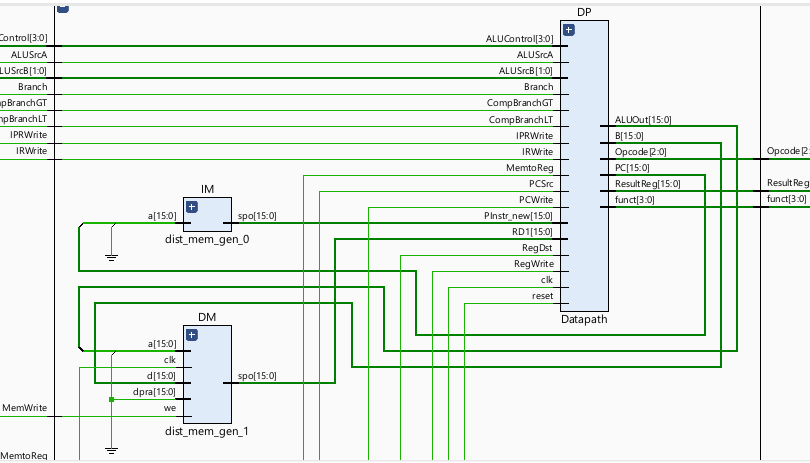
\includegraphics[width=\linewidth]{img/dp_with_mem}
	\caption{\label{fig:final_setup} RTL schematic of Datapath with memories}
\end{figure}
\vspace{2cm}
\subsection{Behavioral simulation:}
\begin{figure}[!htbp]
	\centering
	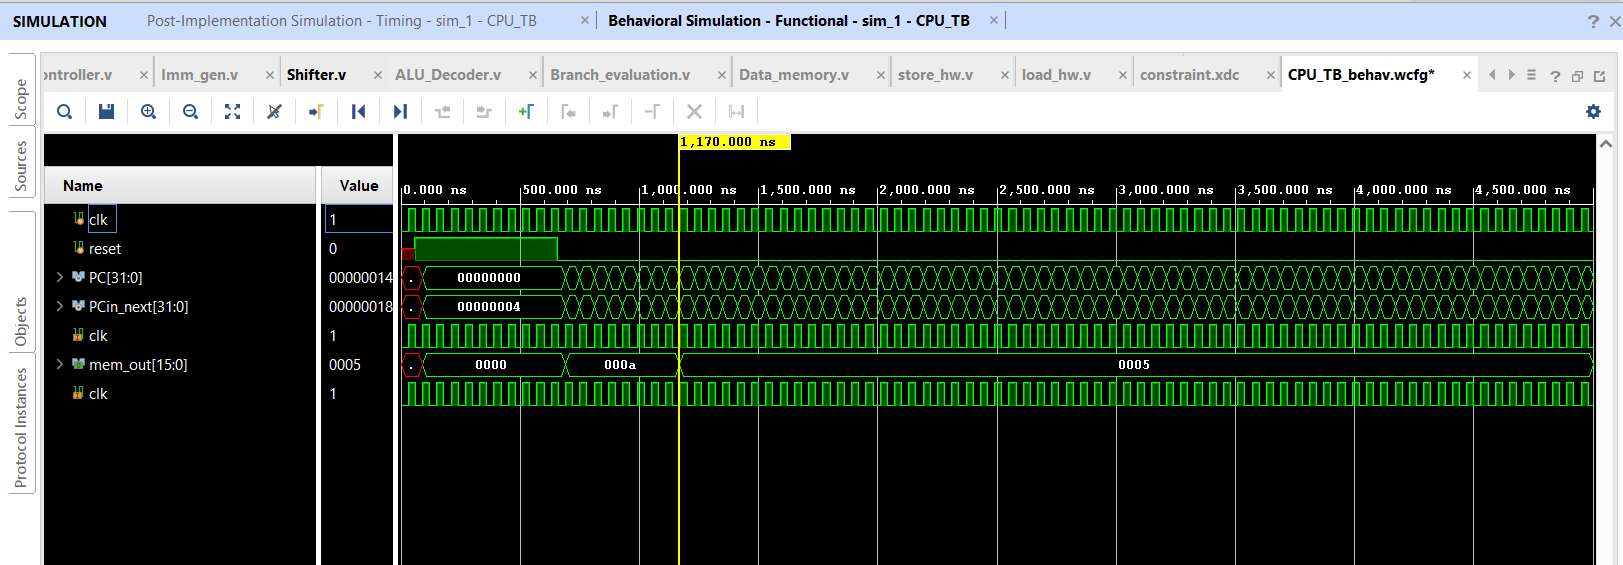
\includegraphics[width=\linewidth]{img/beh_sim}
	\caption{\label{fig:final_setup} : Behavioral simulation of GCD}
\end{figure}
\vspace{2cm}
\subsection{Post implementation timing simulation:}
\begin{figure}[!htbp]
	\centering
	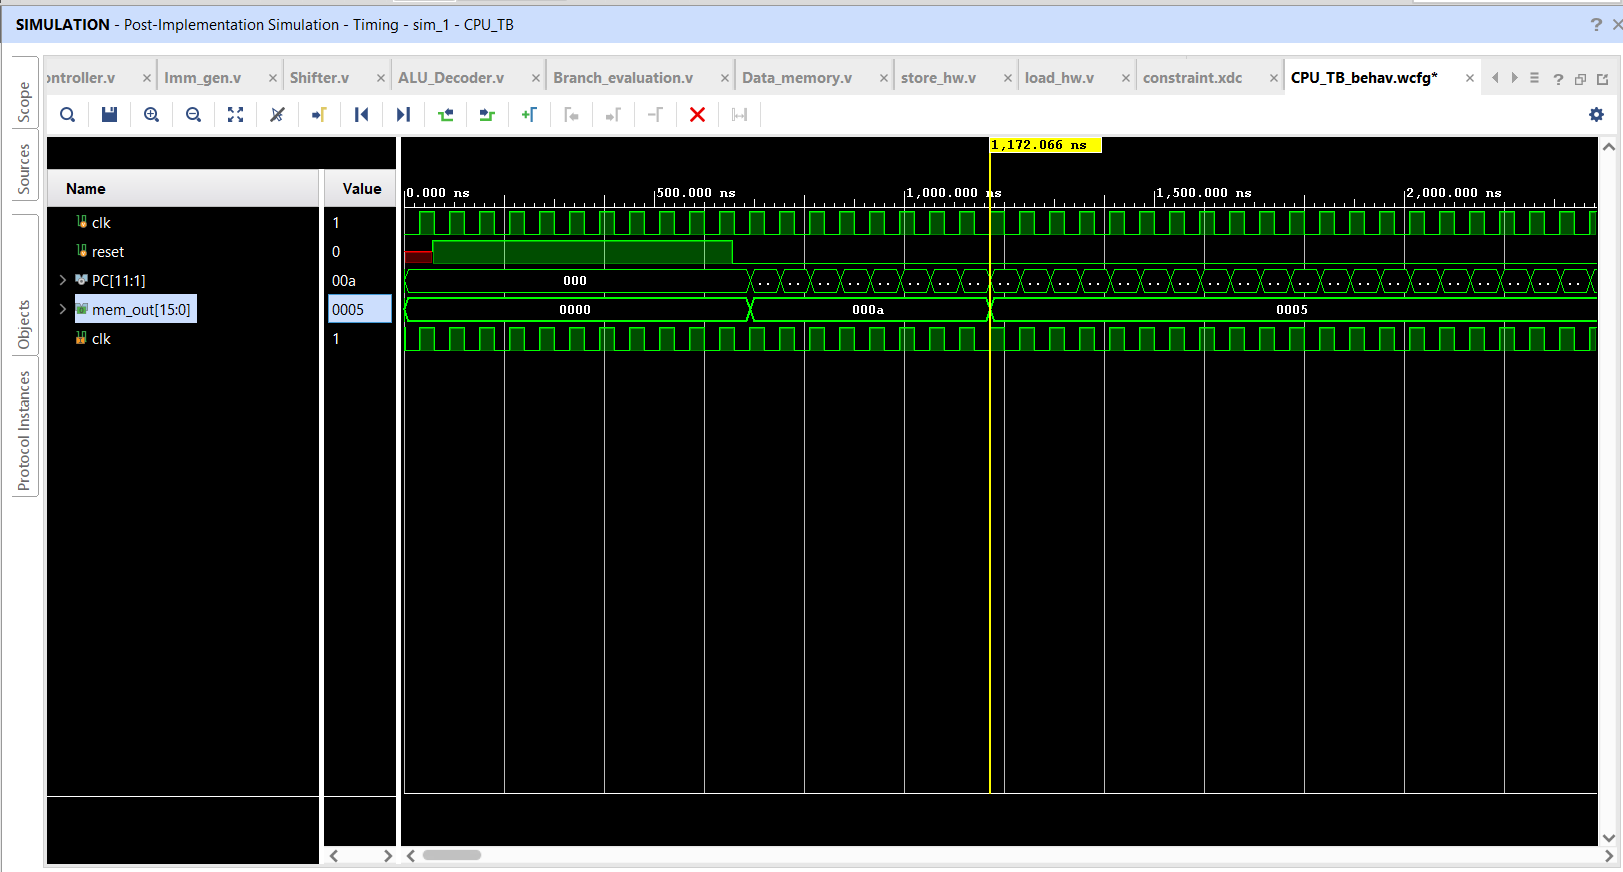
\includegraphics[width=\linewidth]{img/post_imp}
	\caption{\label{fig:final_setup} : Post implementation timing simulation of GCD }
\end{figure}
\vspace{1cm}   
\subsection{Utilization:}
\begin{figure}[!htbp]
	\centering
	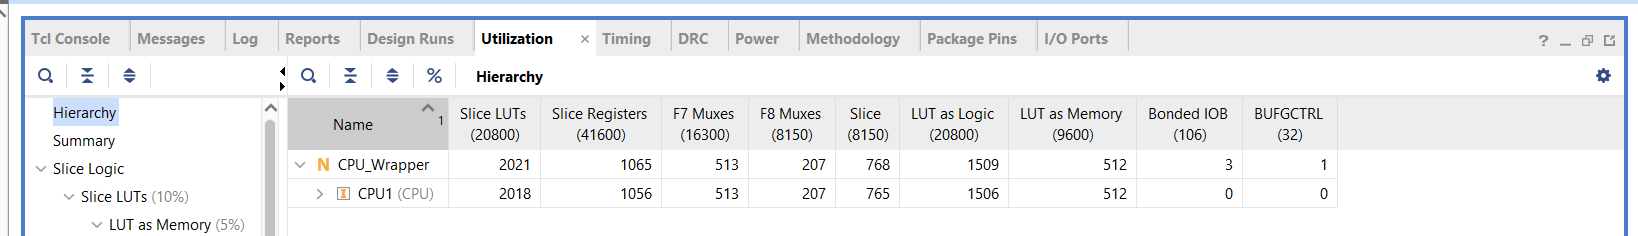
\includegraphics[width=\linewidth,height=0.2\linewidth]{img/utilization}
	\caption{\label{fig:final_setup} :Utilization summary
	 }
\end{figure}
%\begin{figure}[!htbp]
%	\centering
%	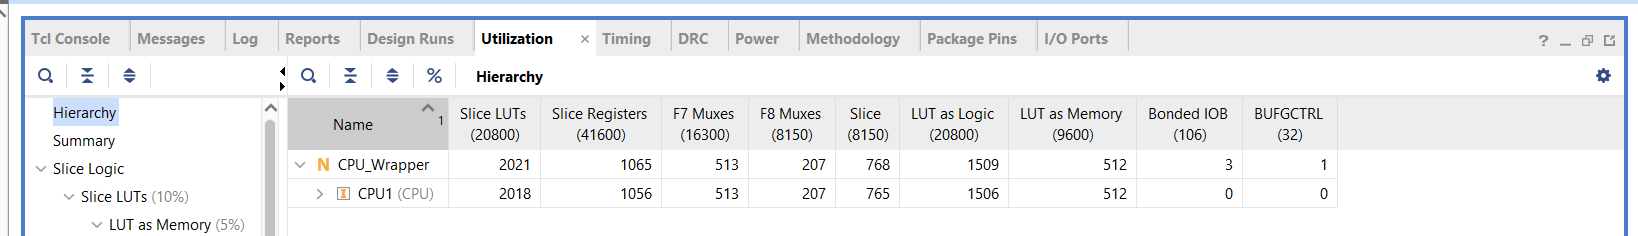
\includegraphics[width=\linewidth]{img/utilization}
%	\caption{\label{fig:final_setup} :Utilization hierarchical distribution
%	}
%\end{figure}

\subsection{Timing summary:}

\begin{figure}[!htbp]
	\centering
	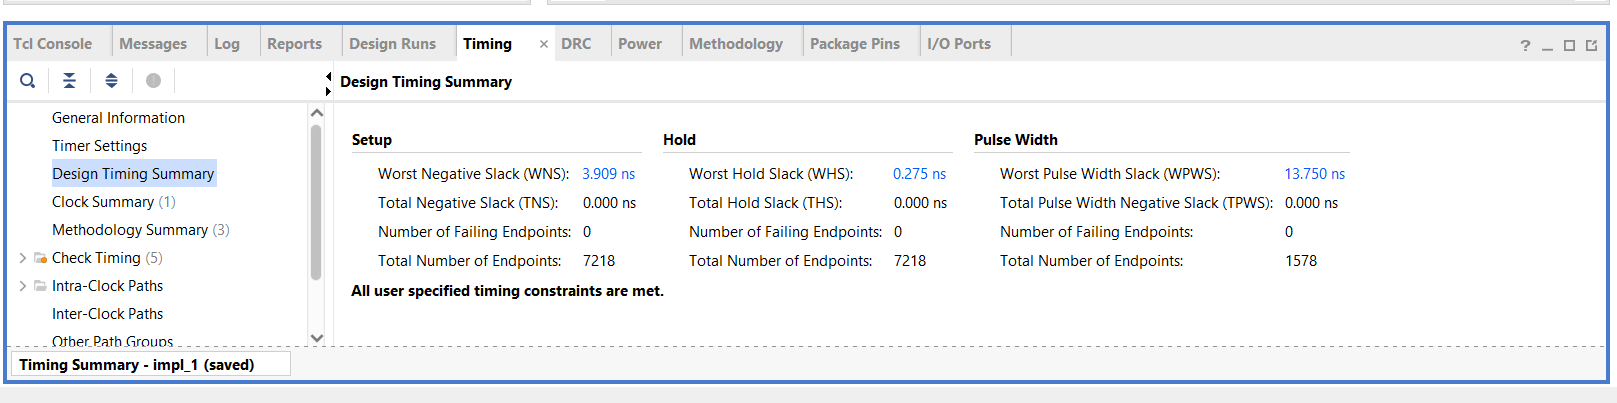
\includegraphics[width=\linewidth,height=0.2\linewidth]{img/timing}
	\caption{\label{fig:final_setup} :Timing Summary
	}
\end{figure}
The minimum time period is calculated as:

\[
\text{Minimum time period} = 30 - 3.9 = 26.1 \, \text{ns}
\]

The maximum frequency is given by:

\[
\text{Maximum frequency} = \frac{1}{26.1 \, \text{ns}} = 38.31 \, \text{MHz}
\]
\vspace{2cm}
\subsection{Power Report:}

\begin{figure}[!htbp]
	\centering
	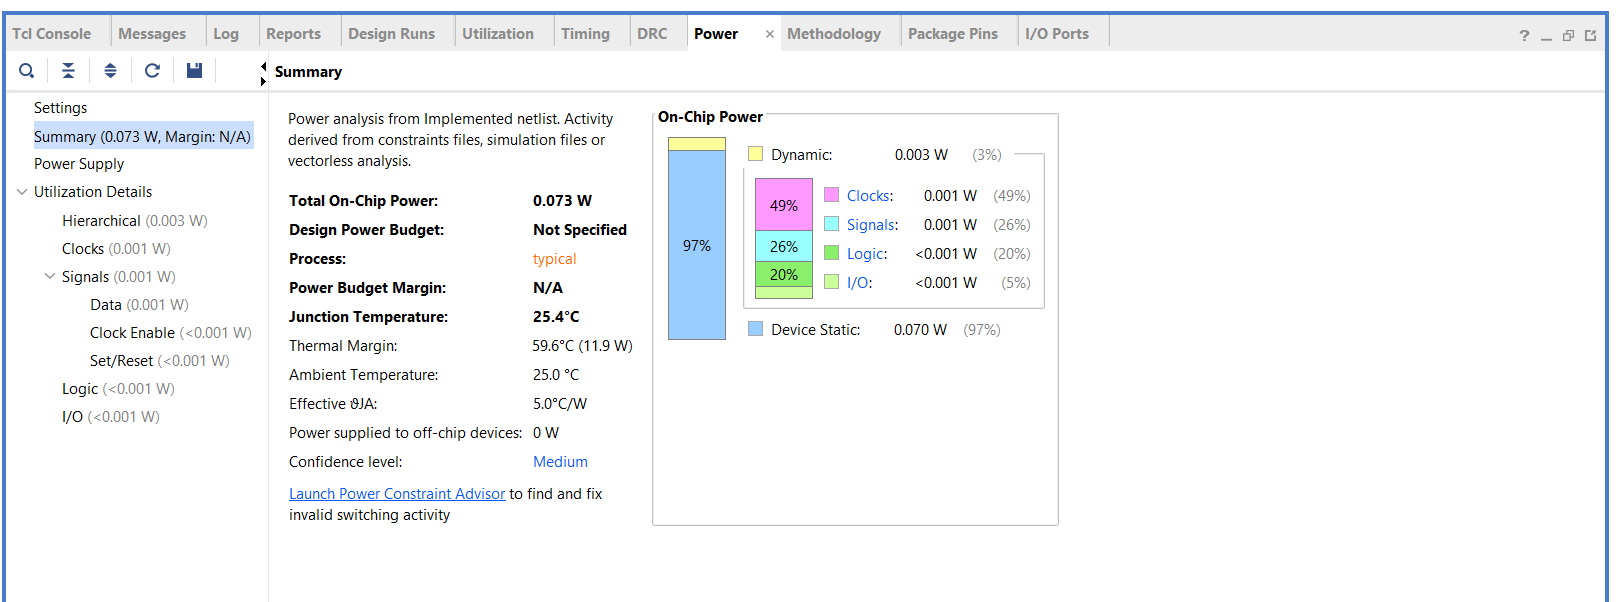
\includegraphics[width=\linewidth]{img/power}
	\caption{\label{fig:final_setup} :Power Report
	}
\end{figure}
%\section{Conclusion}

%In this experiment, the parameters of a DC motor were effectively measured and analyzed. The resistance of the motor was found to be approximately \(1.35 \, \Omega\), and the average inductance was around \(618 \, \mu H\). The designed circuits, including the motor drive, voltage divider, differential amplifier, and Sallen-Key filter, were successfully implemented and provided accurate measurements. The integration of the AMT103 encoder enabled precise speed and position feedback. Overall, the experiment validated the measurement techniques and circuit designs used for motor parameter estimation and control.

%\section{C Code}
%\begin{lstlisting}[language=C]
%	#include <stdint.h>
%	#include <stdbool.h>
%	#include <ctype.h>
%	#include <string.h>
%	#include <stdio.h>
%	#include <math.h>
%	#include "inc\tm4c123gh6pm.h"
%	#include "inc\hw_memmap.h"
%	#include "driverlib\uart.h"
%	#include "user_GPIO.h"
%	#include "user_system.h"
%	#include "ADC.h"
%	#include "PWM.h"
%	#include "driverlib\qei.h"
%	
%	#define PPR 2048 // Pulse per revolution from encoder
%	#define pwm_max 1600 // PWM value for 1KHz
%	#define theta_ref 90000 // 30.000 degrees
%	#define fcpu 16000000 // Clock freq 16MHz
%	#define MAX_POS 8191 //
%	#define edges 4 // Number of edges counted per step
%	#define Ts 0.001 // 1 milli-second (1kHz sampling)
%	#define Ki_1 2 // Current integration gain
%	#define Kp_1 1 // Proportional current gain
%	#define Kp_2 5 // Proportional Gain for omega error
%	#define Ki_2 0.6 // Integral gain for omega error
%	#define Kp_3 1 // Proportional Gain for theta error
%	
%	float Ia_ref, V_ref, int_i, pwm, v, theta, int_v;
%	float error_i, error_v;
%	
%	int moving_avg(int z);
%	void uart_print_num(int x);
%	void qei_init();
%	
%	int temp2, initial_i, ia, count = 0;
%	int dir;
%	
%	int main(void) {
%		// Initialization
%		float temp;
%		int start = 1;
%		int_i = 0;
%		int_v = 0;
%		pwm = 11600;
%		error_v = 0;
%		
%		PORTA_INIT();
%		PORTE_ADC();
%		PWM_init();
%		PortF_Init();
%		UART_config();
%		qei_init();
%		
%		SYSCTL_RCGCGPIO_R |= 0x01;
%		GPIO_PORTA_DIR_R |= (1<<3)|(1<<2); // PA2 and PA3
%		GPIO_PORTA_DEN_R |= (1<<3)|(1<<2);
%		GPIO_PORTA_DATA_R |= (1<<3); // PA3 = 1 and PA2 = 0
%		GPIO_PORTA_DATA_R &= ~(1<<2);
%		
%		// Timer setup - sys tick
%		systick_setup();
%		
%		while (1) {
%			// Main loop
%			freq_factor = sample_ADC(); // Get ADC output
%			temp = (((freq_factor)/4095.0)*3300.0);
%			temp2 = (int)temp;
%			
%			if (start != 0) {
%				initial_i = moving_avg(temp2);
%				start++;
%				if (start == 10) {
%					start = 0;
%				}
%				continue;
%			}
%			
%			ia = moving_avg(temp2);
%			if (state4 == 1) {
%				UARTCharPut(UART0_BASE, '\t');
%				printstring("Position in Degrees = ");
%				uart_print_num(theta);
%				UARTCharPut(UART0_BASE, 13);
%				UARTCharPut(UART0_BASE, 10);
%				state4 = 0;
%				count = 0;
%			}
%			delayMs(1);
%		}
%	}
%	
%	int moving_avg(int z) {
%		static int prev_z[10];
%		static int index;
%		float avg = 0;
%		int i;
%		if (index >= 10)
%		index = 0;
%		prev_z[index] = z;
%		index++;
%		
%		for (i = 0; i < 10; i++) {
%			avg += prev_z[i]; // Corrected averaging calculation
%		}
%		
%		return (int)(avg / 10.0);
%	}
%	
%	void SysTick_Handler(void) {
%		theta = (360000*QEI0_POS_R)/MAX_POS; // theta measured by QEI
%		dir = (QEI0_STAT_R & 0x02); // Extract direction
%		v = ((100*QEI0_SPEED_R*60)/(PPR*edges)); // Velocity in RPM
%		
%		// Velocity control loop
%		V_ref = (theta_ref - theta) * Kp_3 / 1000;
%		if (V_ref < 0) V_ref = -V_ref;
%		if (V_ref > 400) V_ref = 400;
%		error_v = V_ref - v;
%		
%		int_v += error_v * Ts * 10; // Velocity integration
%		if (int_v > 5000) int_v = 5000;
%		else if (int_v < -5000) int_v = -5000;
%		
%		// Current control loop
%		Ia_ref = (Ki_2 * int_v + Kp_2 * error_v); // Current reference
%		error_i = Ia_ref - ia;
%		
%		int_i += error_i * Ts; // Integration
%		if (int_i > 3000) int_i = 3000;
%		else if (int_i < -4000) int_i = -4000;
%		
%		// PWM update
%		if (dir == 2) {
%			pwm = pwm_max/2 - (Ki_1 * int_i + Kp_1 * error_i);
%		} else if (dir == 0) {
%			pwm = pwm_max/2 - (Ki_1 * int_i + Kp_1 * error_i);
%		}
%		
%		if (pwm > 0.8 * pwm_max) pwm = 0.8 * pwm_max;
%		else if (pwm < 0.05 * pwm_max) pwm = 0.05 * pwm_max;
%		
%		PWM1_1_CMPA_R = pwm;
%		count++;
%		if (count >= 1000) {
%			state4 = 1;
%			count = 0;
%		}
%	}
%	
%	void qei_init() {
%		SYSCTL_RCGCQEI_R |= 0x01; // QEI run mode clock gating control on
%		SYSCTL_RCGCGPIO_R |= 0x08; // Enable clock for PORTD
%		GPIO_PORTD_LOCK_R = 0x4C4F434B; // Unlock port D
%		GPIO_PORTD_CR_R |= 0xC8; // Allow changes
%		GPIO_PORTD_AMSEL_R &= 0x00; // Disable analog function
%		GPIO_PORTD_DEN_R |= 0xC8; // Enable Digital Pins
%		GPIO_PORTD_DIR_R &= ~0xC8; // Configure pins as Input
%		GPIO_PORTD_AFSEL_R |= 0xC8; // QEI alternate function
%		GPIO_PORTD_PCTL_R = (GPIO_PORTD_PCTL_R & 0x00FF0FFF) + 0x66006000;
%		QEI0_CTL_R |= ((1 << 5) | (1 << 4) | (1 << 3)); // Enable velocity capture
%		QEI0_MAXPOS_R |= MAX_POS;
%		QEI0_LOAD_R = (fcpu * 0.01); // Update speed every 10ms
%	}
%	
%	void uart_print_num(int x) {
%		int temp;
%		int n_flag = 0;
%		int count = 1;
%		if (x < 0) {
%			x = -1 * x;
%			n_flag = 1;
%		}
%		
%		temp = x;
%		if (temp == 0) {
%			UARTCharPut(UART0_BASE, '0');
%			return;
%		}
%		
%		while (temp / 10 != 0) {
%			temp = temp / 10;
%			count = count * 10;
%		}
%		
%		temp = x;
%		if (n_flag == 1) {
%			UARTCharPut(UART0_BASE, '-');
%		}
%		
%		while (count != 0) {
%			UARTCharPut(UART0_BASE, '0' + temp / count);
%			temp = temp % count;
%			count = count / 10;
%		}
%	}
%\end{lstlisting}

%\section{Conclusions}
%
%In most cases, the experimental results will not match theoretical
%calculations. This sections addresses this by discussion on these
%mismatches. This is a very important section. It provides an insight
%into the authors' thought flow. Note that this section is not merely
%a summary of the entire article. It discusses the experiment from
%the angle of practicalities and uncertainities. As there are no ideal
%situations in practical realisations, the authors should discuss on
%aspects where the result is not as expected by theory. In what ways
%the short comings in the theory can be addressed? What are the possible
%solutions? Brainstorming is an essential component of this section.
%The authors can also put forth comparisons based on similar circuits,
%simulation results and discussions in literature to consolidate the
%results that have been obtained in this experiment.

%\bibliographystyle{unsrt}
%\bibliography{report}

\end{document}
